En este capítulo, se introduce una aplicación web diseñada para interactuar con el \textit{datalogger} descrito en el capitulo anterior. Esta herramienta de software simplifica la carga de metadatos esenciales, incluyendo la información de los sensores de referencia y los sensores bajo calibración, los certificados de calibración y las especificaciones de la zona de medición del túnel de viento. La aplicación ofrece la posibilidad de configurar el \textit{datalogger}, definiendo la interfaz eléctrica de los anemómetros, los intervalos de muestreo y procesamiento de datos, y los puntos de medición de la velocidad del viento. Además, permite establecer los tiempos de crecimiento y el periodo de estabilidad en cada punto de medición Una vez configurado el sistema, el software inicia el proceso de medición de los sensores y simultáneamente, se envían referencias de velocidad del viento al controlador PID, el cual, ajusta la velocidad del viento al valor deseado. Las mediciones obtenidas son verificadas por el operador y, si son correctas, el software procede a calcular la incertidumbre expandida de cada punto de viento medido. Los resultados se presentan mediante gráficos y tablas, que a su vez, se almacenan en una base de datos y pueden descargarse para emitir el certificado de calibración correspondiente.


%%%%%%%%%%%%%%%%%%%%%%%%%%%%%%%%%%%%%%%%%%%%%%%%%%%%%%%%%%%%%%%%%%%%%%%%%%%%%%%%%%%%%%%%%%%%%%%%%%%%%%%%%%%%%%%%%%%%%%%%
\section{Desarrollo de la aplicación WEB}
% hablar de las herramientas utilizadas para todo el desarrollo, contar todo, los entornos, lenguajes y frameworks etc
Durante el desarrollo de la aplicación web, se emplearon diversas herramientas para llevar a cabo el proyecto de manera eficiente. Se utilizó Django en su versión 4.2 como \textit{framework} principal, junto con Python 3.10, proporcionando una base sólida y flexible para el desarrollo \textit{back end}. Para la gestión de la base de datos, se optó por PostgreSQL en su versión 15 y se utilizó PGAdmin 4 para gestionar dicha base de datos. La conexión entre Django y PostgreSQL se realizó utilizando PSYCOPG2 en su versión 2.9.5. En el desarrollo de \textit{front end}, se emplearon JavaScript y jQuery para hacer la página web dinámica y permitir la visualización de datos actualizados en tiempo real. También se utilizaron HTML y CSS para estructurar y estilizar el contenido de la aplicación web. Además, se emplearon herramientas como NumPy 1.24.2, SciPy  1.11.2 para el procesamiento de datos y Plotly 5.15 para generar gráficos dinámicos, así como Pandas 2.2 para la manipulación de datos. Toda la aplicación corre en un servidor local, de la Figura \ref{fig:sistemaDesarrollado}, dentro de un entorno virtual de Python para mantener las dependencias aisladas y facilitar la portabilidad del proyecto a otros entornos. Se gestionó el control de versiones con Git y GitHub, en un repositorio \cite{AppWebInstrumentalSMN2024}, subiendo el código y trabajando en distintas ramas para luego integrar los cambios en la rama principal, lo que permitió mantener un historial claro de los cambios realizados.
%%%%%%%%%%%%%%%%%%%%%%%%%%%%%%%%%%%%%%%%%%%%%%%%%%%%%%%%%%%%%%%%%%%%%%%%%%%%%%%%%%%%%%%%%%%%%%%%%%%%%%%%%%%%%%%%%%%%%%%%
\subsection{Arquitectura del software}
Para desarrollar la aplicación, se utilizó una arquitectura de cinco capas, como se muestra en la Figura \ref{fig:arquitecturaSoft}. La primera capa está conformada por el servidor web Nginx, que actúa como un servidor \textit{proxy} inverso. Nginx se encarga de manejar las solicitudes HTTP entrantes, distribuyéndolas eficientemente y proporcionando un equilibrio de carga, además de brindar contenido estático como archivos HTML, CSS, JavaScript e imágenes. Esta capa permite mejorar el rendimiento y la seguridad de la aplicación al filtrar y dirigir el tráfico de manera óptima. La segunda capa está compuesta por Gunicorn, un servidor WSGI (\textit{Web Server Gateway Interface}) que sirve como intermediario entre Nginx y la aplicación web desarrollada en Django. Gunicorn se encarga de gestionar los procesos de la aplicación, proporcionando un entorno escalable y capaz de manejar múltiples solicitudes concurrentes. Esta capa es crucial para asegurar que la aplicación pueda responder de manera rápida y eficiente a las demandas de los usuarios. En la tercera capa se encuentra la aplicación web desarrollada en Django, un \textit{framework} de alto nivel que facilita el desarrollo rápido y eficiente de aplicaciones web seguras y mantenibles.  Esta capa es responsable de la lógica de negocio de la aplicación, la gestión de las bases de datos y la interacción con los usuarios a través de interfaces web dinámicas. La cuarta capa está constituida por el sistema de gestión de bases de datos PostgreSQL, encargado del almacenamiento y recuperación de datos de manera eficiente y segura. La integración con Django se realiza a través de su ORM (\textit{Object-Relational Mapping}), que permite interactuar con la base de datos utilizando objetos en Python. Esto permite crear registros, guardar información y realizar consultas de manera sencilla, traduciendo automáticamente las operaciones en Python a consultas SQL en la base de datos. Finalmente, la quinta capa consiste en un servidor \textit{WebSocket}, como se describió en la sección \ref{sec:serverWebSocket}. Este protocolo de comunicación basado en HTTP permite que tanto los clientes como el sistema embebido se conecten con la aplicación web, logrando una comunicación bidireccional en tiempo real. Esta capa es esencial para aplicaciones que requieren actualizaciones en tiempo real y una interacción continua con dispositivos de hardware.

\begin{figure}[H]
    \centering
    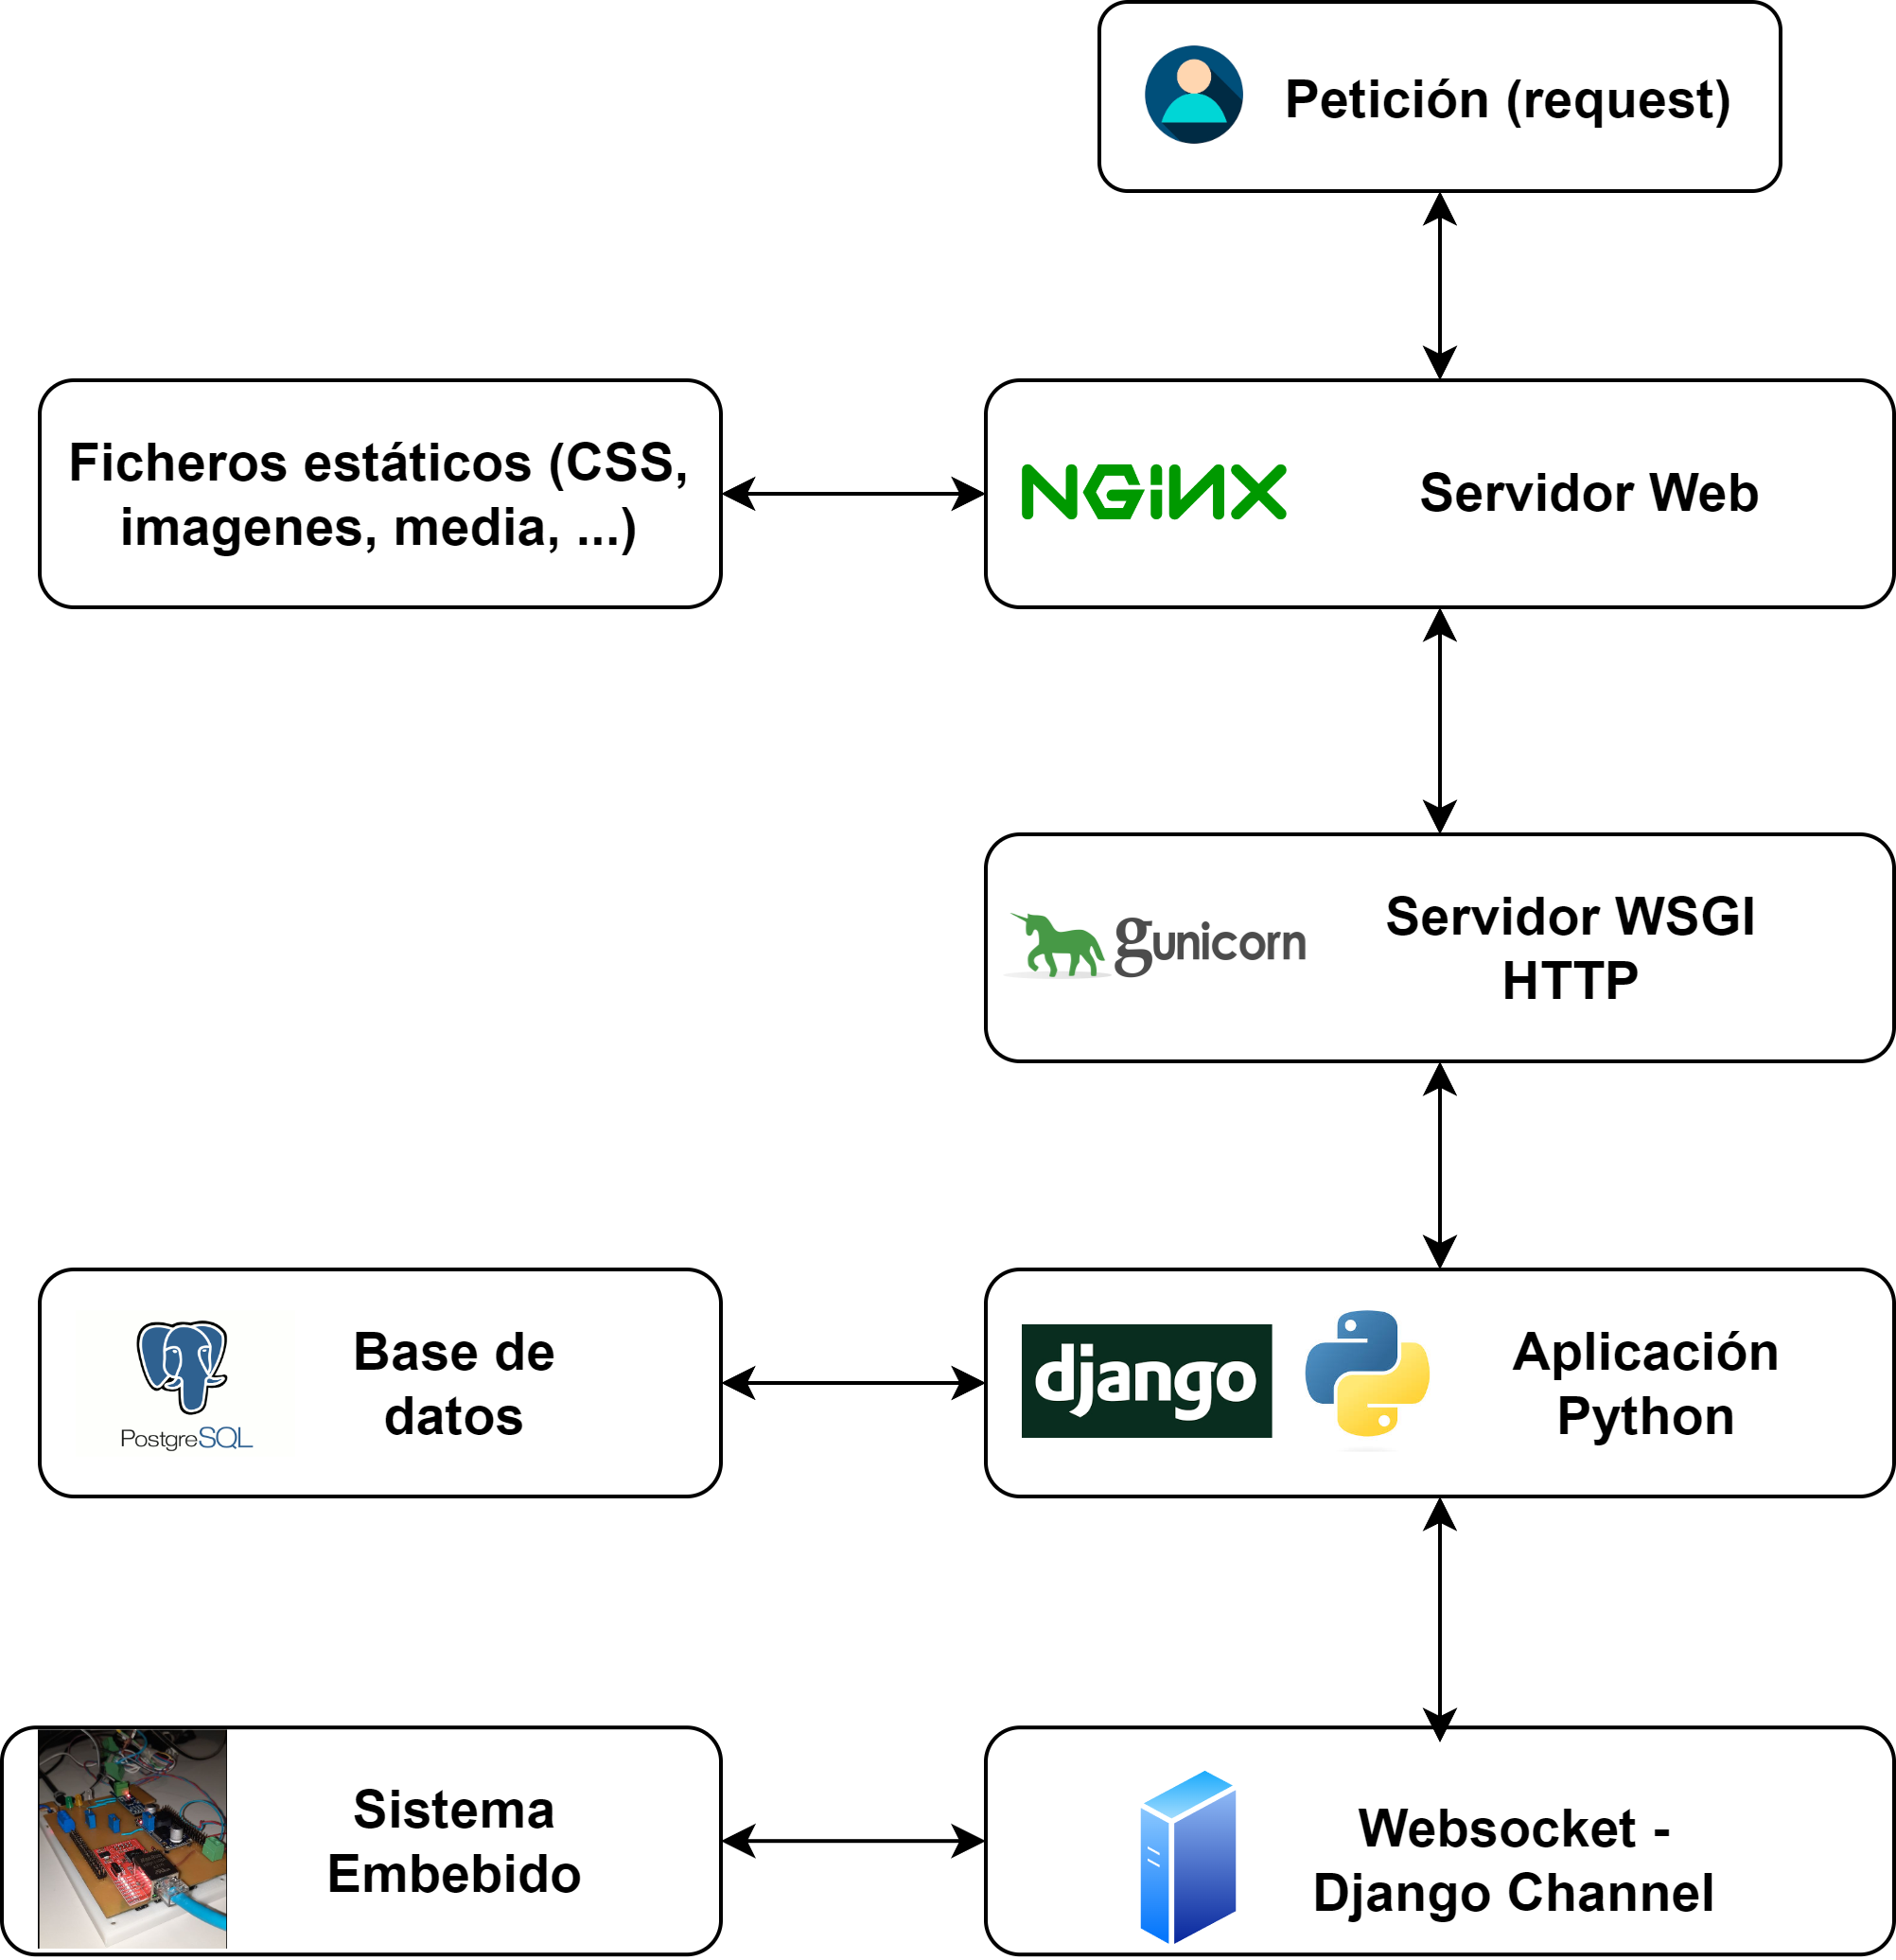
\includegraphics[width=1\linewidth]{Figuras/AplicacionWeb/arquitecturaSoft.png}
    \caption{Arquitectura del software implementada.}
    \label{fig:arquitecturaSoft}
\end{figure}

\subsection{Patron de diseño de software}
Se empleó el patrón de diseño MVT (Modelo-Vista-Plantilla), ilustrado en la Figura \ref{fig:patronMVT}. Este patrón es ampliamente utilizado en el desarrollo web con el \textit{framework} de trabajo Django. El patrón MVT permite una distinción explícita de las responsabilidades, permitiendo dividir el problema en módulos , lo que facilita tanto el desarrollo como el mantenimiento del código. 

\begin{itemize}
    \item \textbf{Modelo (M)}: Representa la capa de acceso a la base de datos (ORM). Contiene toda la información sobre los datos, cómo acceder a ellos, validarlos, su comportamiento y las relaciones entre ellos.
    \item \textbf{Vista (V)}:  Corresponde a la capa de lógica de negocios. Se encarga de procesar las solicitudes del navegador y recuperar los datos necesarios del modelo. Luego, renderiza la plantilla (template) para mostrar el HTML resultante.
    \item \textbf{Template (T)}: (Plantilla), representa la capa de presentación, es la parte visual de la aplicación. El template integra los datos dinámicos recuperados del modelo y genera el HTML final que se envía al navegador.

\end{itemize}
\begin{figure}[H]
    \centering
    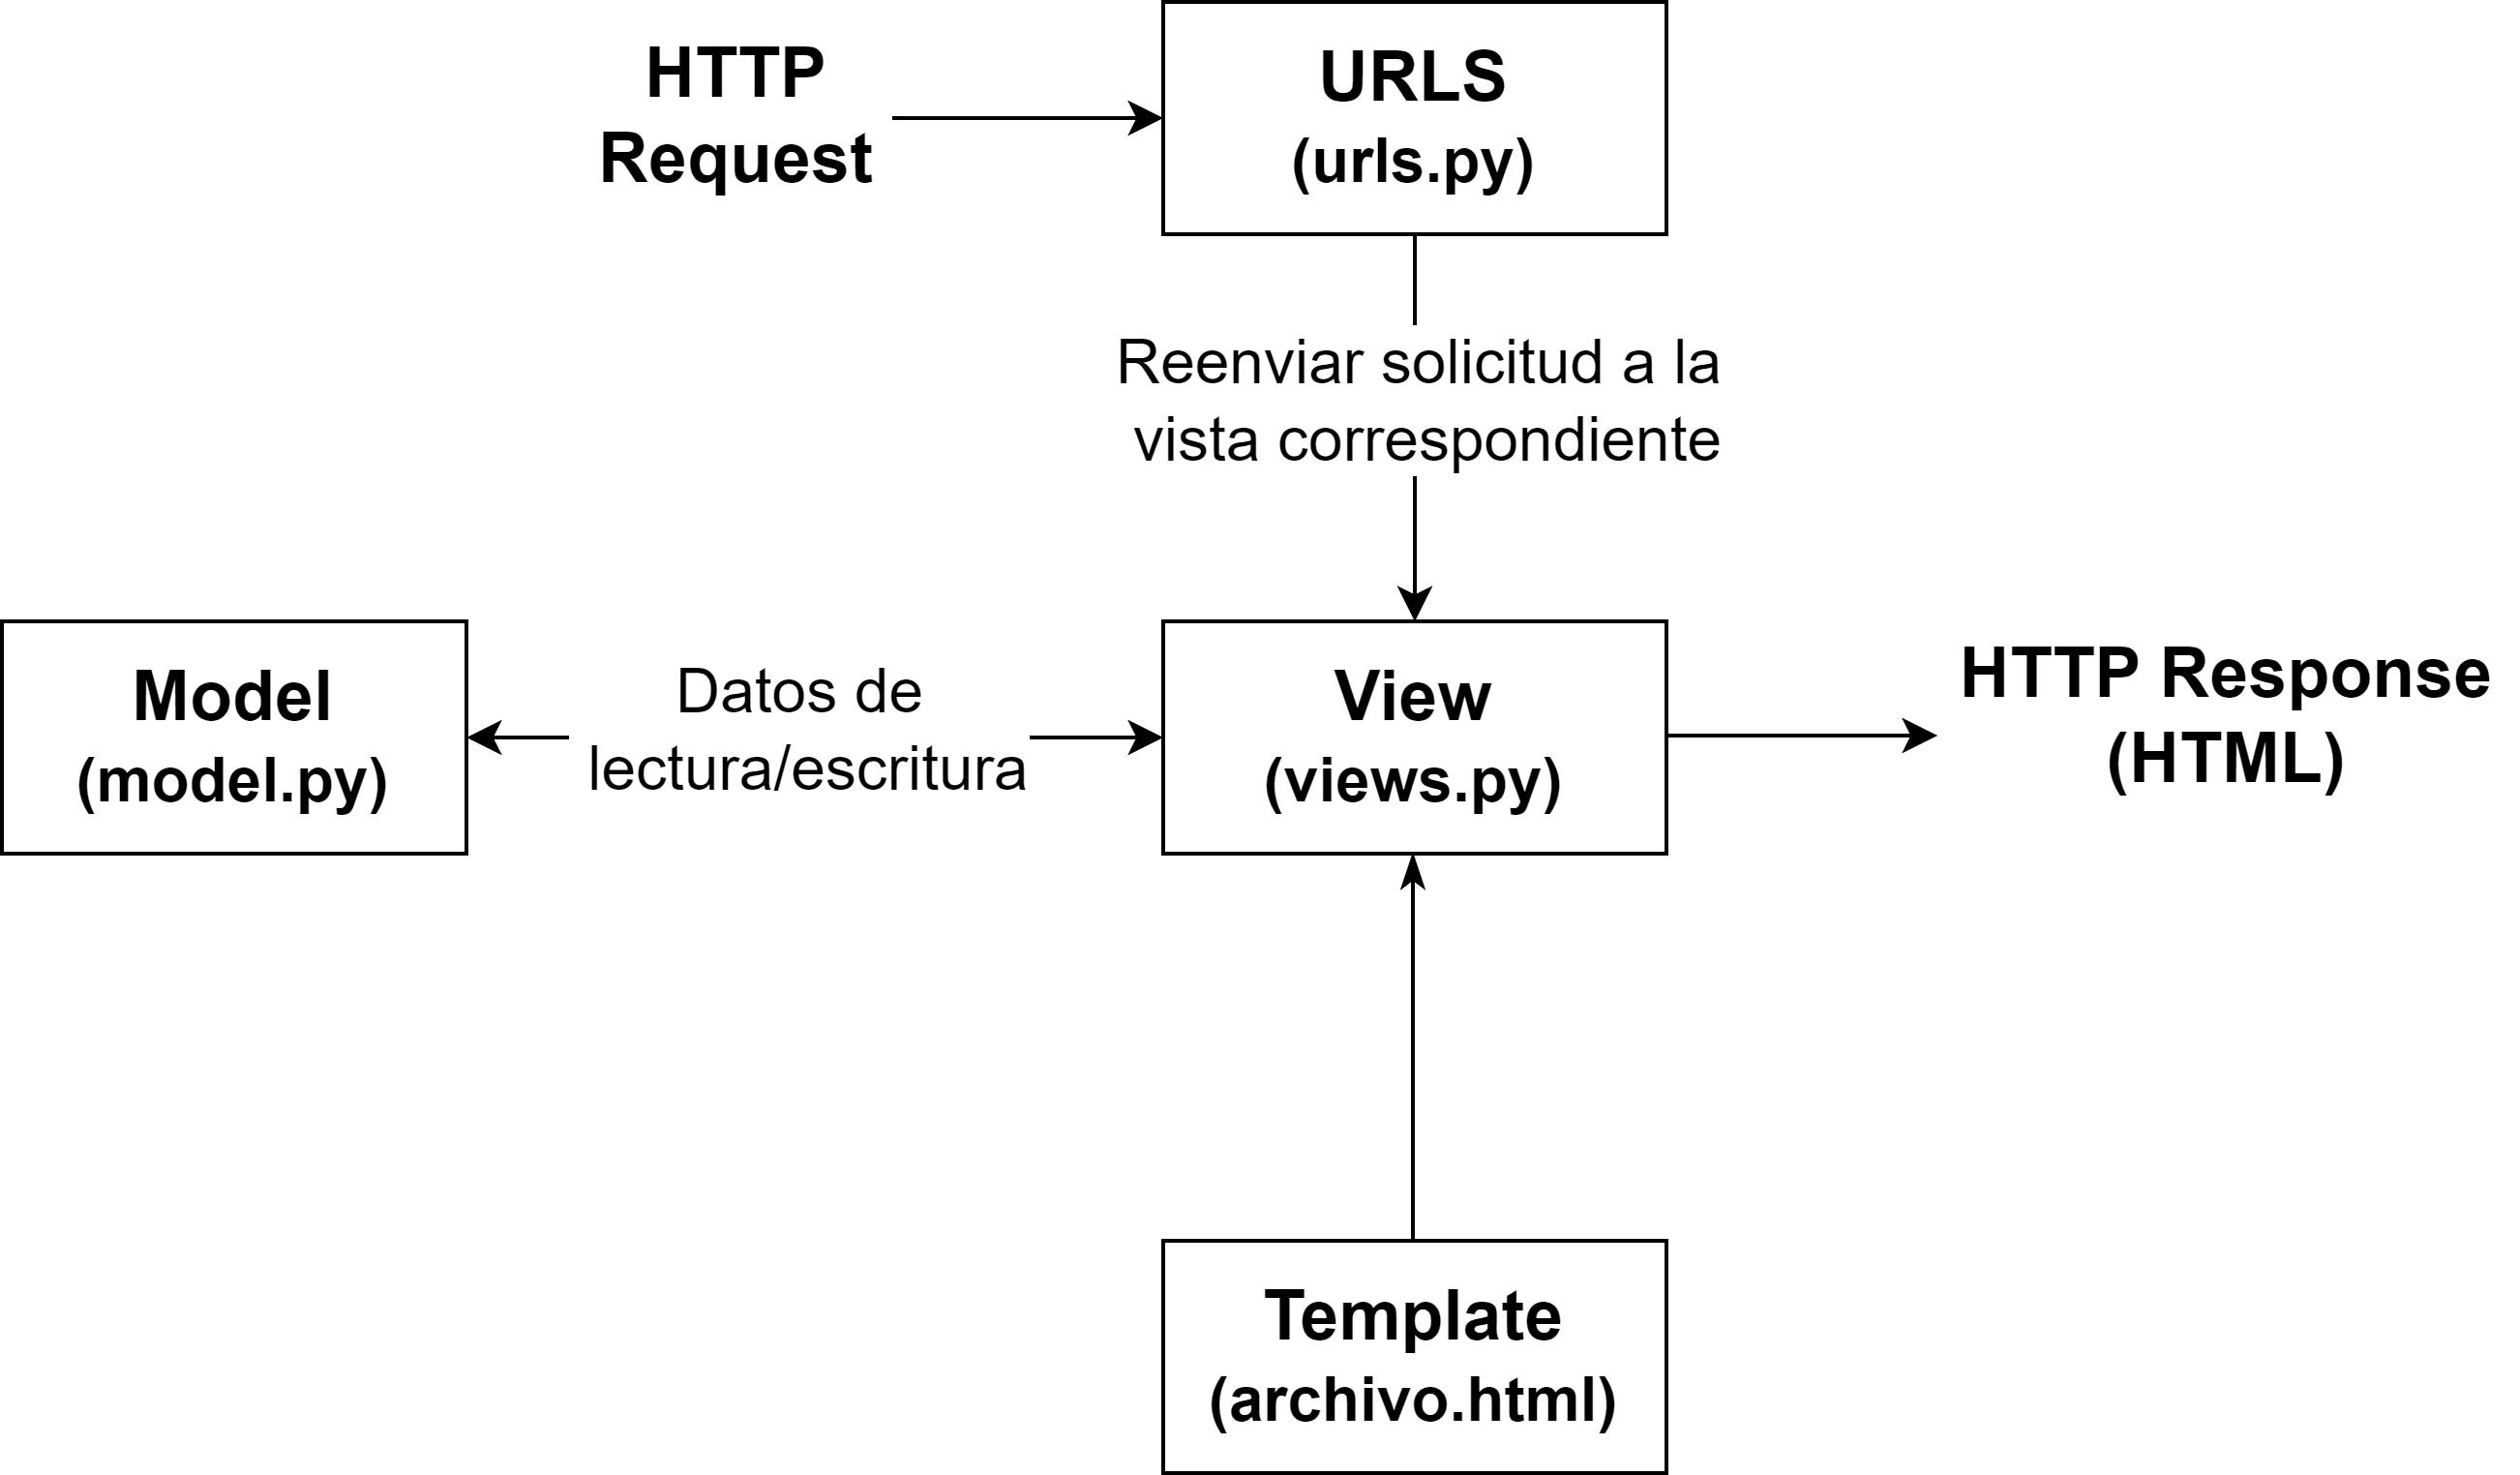
\includegraphics[width=0.8\linewidth]{Figuras/AplicacionWeb/patronMVT.png}
    \caption{Patrón de diseño de software MVT, que divide la lógica del programa en cuatro elementos interconectados.}
    \label{fig:patronMVT}
\end{figure}

%%%%%%%%%%%%%%%%%%%%%%%%%%%%%%%%%%%%%%%%%%%%%%%%%%%%%%%%%%%%%%%%%%%%%%%%%%%%%%%%%%%%%%%%%%%%%%%%%%%%%%%%%%%%%%%%%%%%%%%%
\subsection{Back End}\label{sec:back_end}
% (POnerlo como parrafo, en terminos generales el Back End se encarga de .... (seccion \ref{poner la que corresponda en funcion de como lo menciona}))
% El \textit{back end} se encarga de:
% \begin{itemize}
%     \item Administrar la base de datos, incluyendo la ejecución de consultas, la realización de actualizaciones y la aplicación de validaciones para garantizar la integridad y consistencia de la información.
%     \item Recibir o gestionar solicitudes HTTP y conexiones al servidor \textit{WebSocket}.
%     \item Enviar comandos de configuración hacia el \textit{datalogger} y gestionar la recepción de mediciones de los sensor.
%     \item Generar un perfil de referencias de velocidad de viento almacenadas en la base de datos, que se van a transmitir al \textit{datalogger} para controlar el motor del túnel.
%     \item A partir de las mediciones crudas de velocidades de viento, calcular el presupuesto de incertidumbre de la corrección.
% \end{itemize}

El \textit{back end} se encarga de administrar la base de datos, incluyendo la ejecución de consultas, la realización de actualizaciones y la aplicación de validaciones para garantizar la integridad y consistencia de los datos. Además, gestiona las solicitudes HTTP y las conexiones con el servidor \textit{WebSocket}. También envía comandos de configuración hacia el \textit{datalogger} y se encarga de la  recepción de mediciones de los sensores. Por otro lado, genera un perfil de referencias de velocidad de viento que se transmiten al \textit{datalogger} para controlar el motor del túnel. Finalmente, a partir de las mediciones crudas de velocidades de viento, almacenadas en la base de datos, se calcula el presupuesto de incertidumbre para cada valor de viento configurado.

\subsubsection{Base de datos}

Dado que la aplicación está diseñada para manejar una gran cantidad de datos que requieren almacenamiento y una recuperación eficiente, se ha implementado una base de datos relacional. El diagrama presentado en la figura \ref{fig:DiagramaSimplificadoBd}, ilustra la estructura de la base de datos. Esta estructura incluye diversas tablas que almacenan información crucial para la aplicación. Entre estas tablas se encuentran las que registran los datos del sensor patrón y el sensor bajo calibración, así como los detalles relacionados con el certificado de calibración del patrón. Además, se documentan los registros del certificado de caracterización del túnel de viento. También se incluye información sobre la configuración del \textit{datalogger} y del túnel de viento.
\begin{figure}[H]
    \centering
    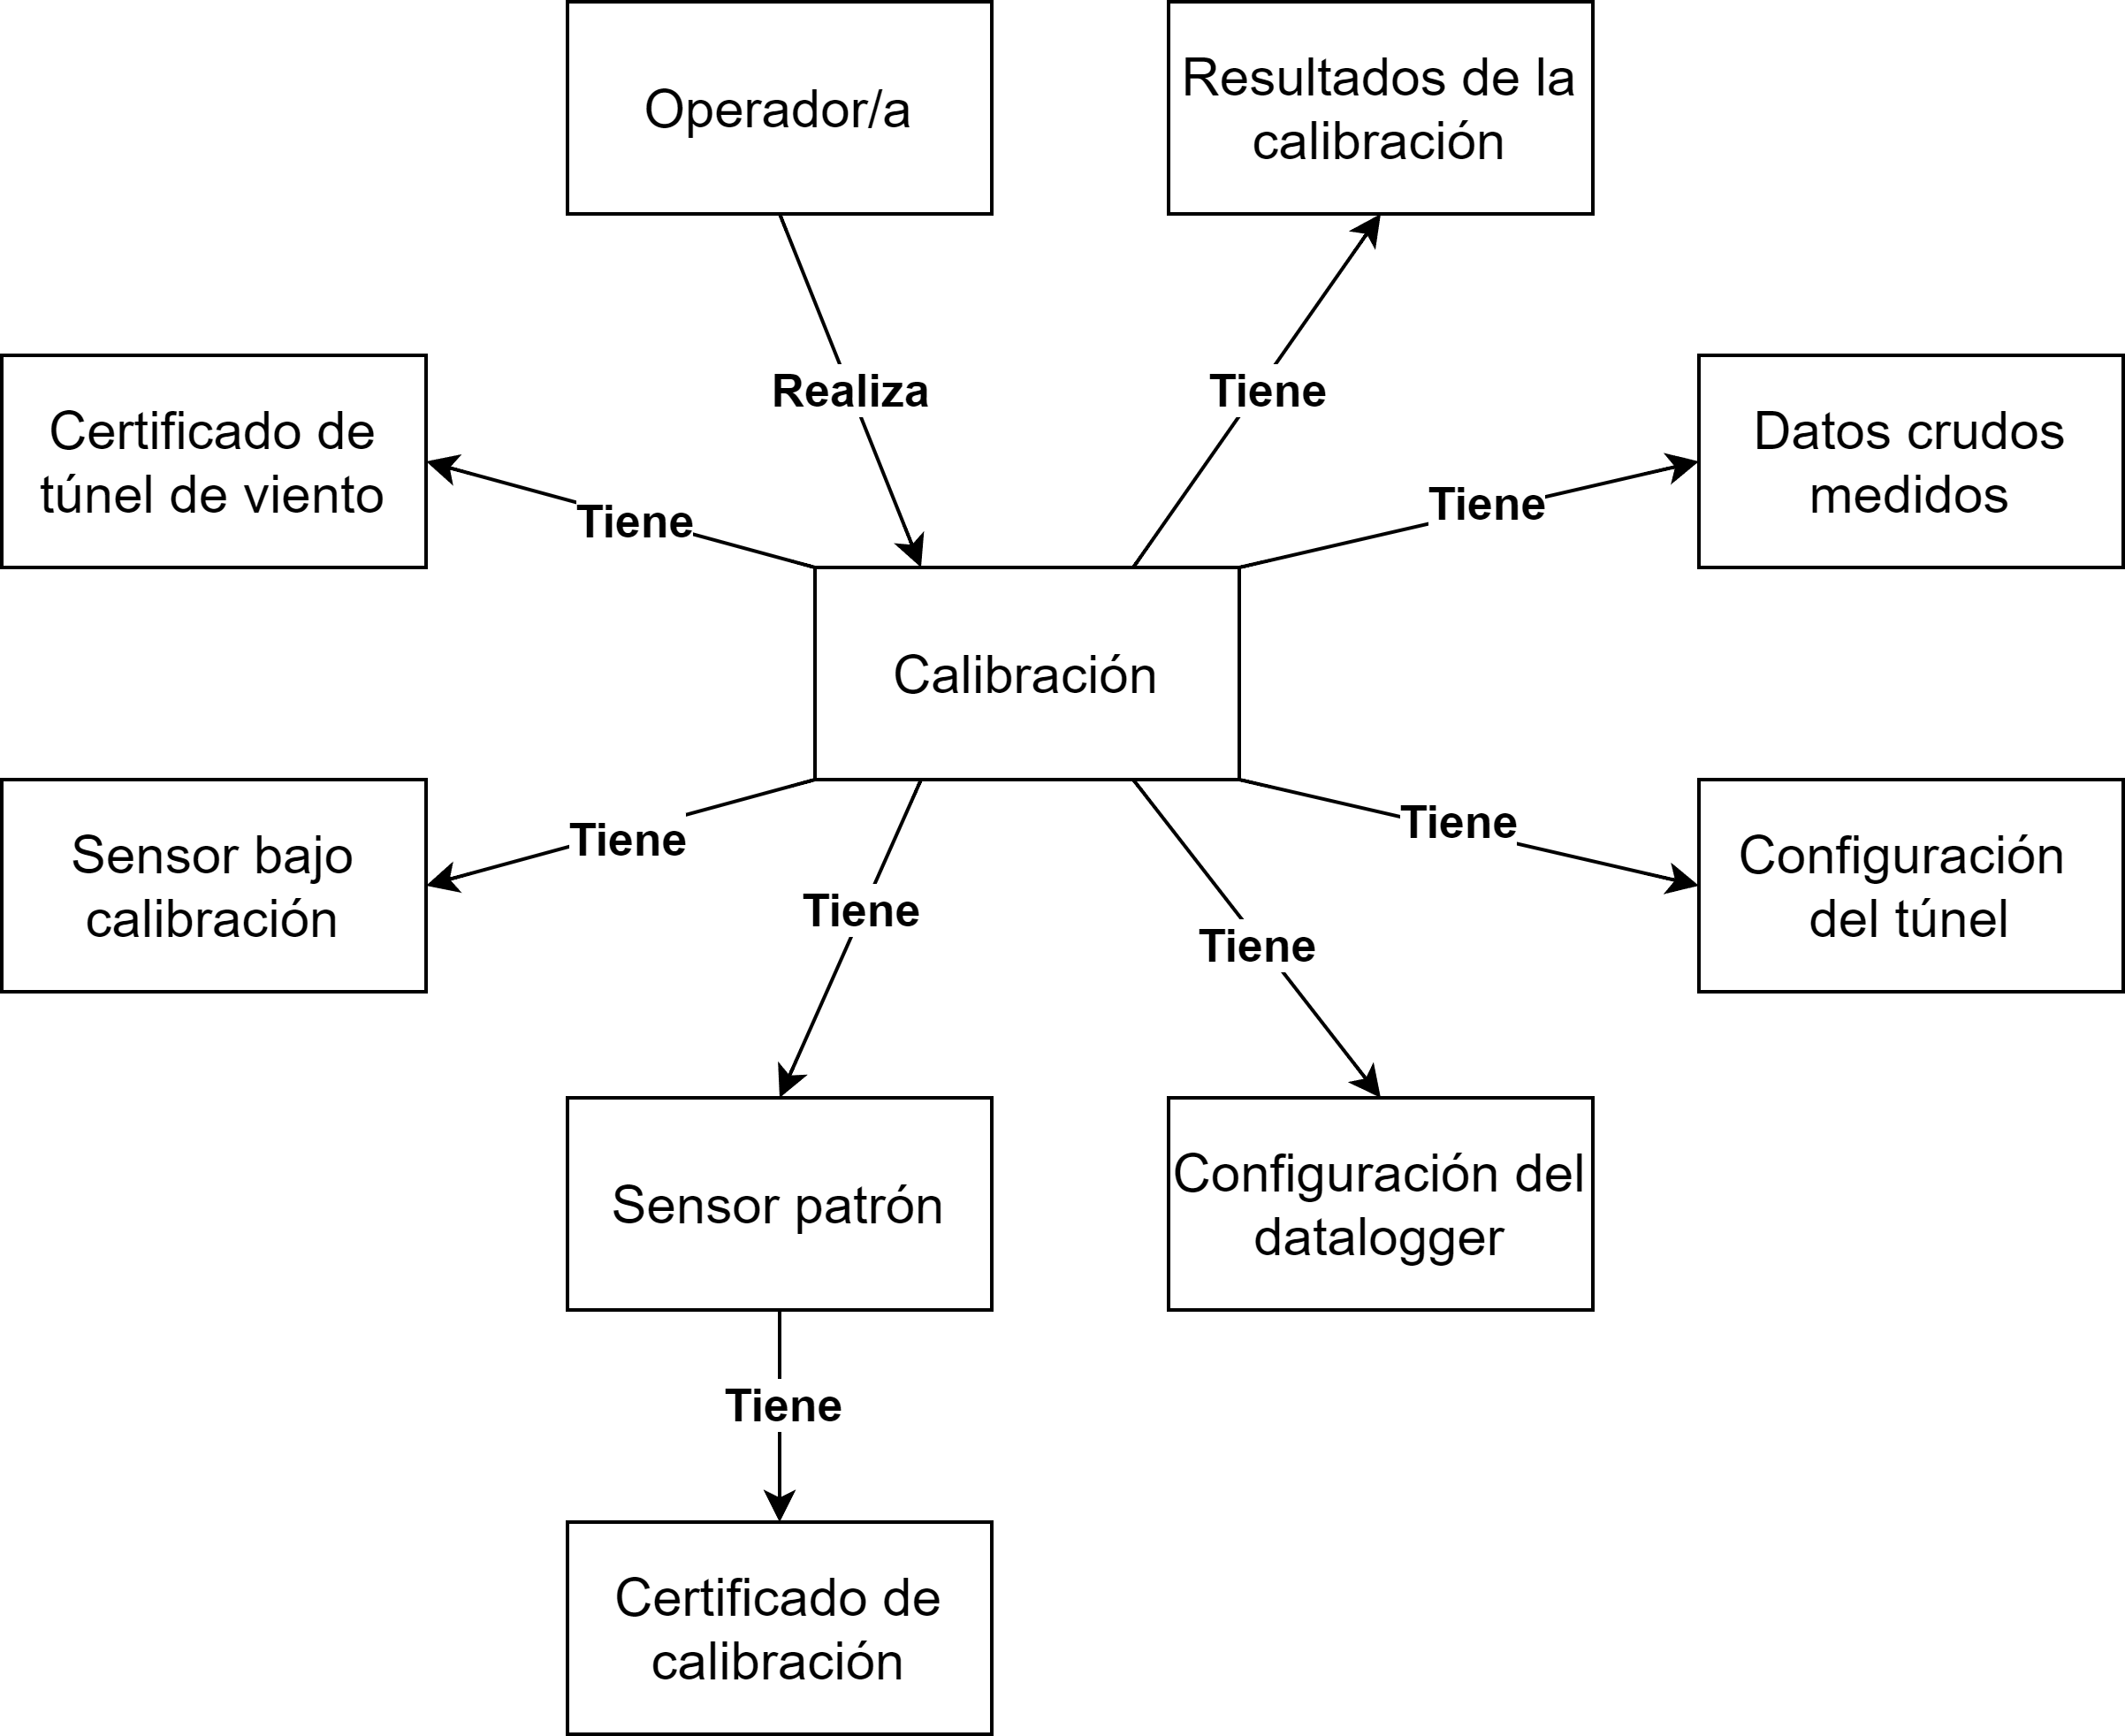
\includegraphics[width=0.8\linewidth]{Figuras/AplicacionWeb/backend/DiagramaSimplificadoBd.png}
    \caption{Diagrama de tablas diseñada para la aplicación Web.}
    \label{fig:DiagramaSimplificadoBd}
\end{figure}

Cuando se inicia una calibración y se empiezan a recibir datos de los sensores, toda esta información se almacena en una tabla definida como \texttt{DatosMedidos} de la base de datos. Asimismo, se guardan los resultados generados antes y después del procesamiento de los datos. Todas estas tablas están relacionadas mediante claves foráneas (relación de uno a muchos) con la tabla \texttt{Calibración}. Esto se debe a que una calibración está asociada a un único \textit{datalogger} o a un único sensor IBC, y se puede recuperar la información de esa  calibración a través de un numero identificador definido como su clave primaria. En la Figura \ref{fig:DiagramaEntidadrelacion} se ve el diagrama de entidad relación donde se describe con más detalle las tablas, los atributos de tabla con su tipo de dato, las claves primarias y las claves foráneas.


% Todo las definiciones de estas tablas se realizaron a traves de clases usando el Conector de ORM de django con la base de datos Postggre SQL, a traves de la definir una clase que hereda de models.Model, como se ve en el codigo \ref{}, donde se define la clase,  ConfigTunel
%%%%%%%%%%%%%%%%%%%%%%%%%%%%%%%%%%%%%%%%%%%%%%%%%%%%%%%%%%%%%%%%%%%%%%%%%%%%%%%%%%%%%%%%%%%%%%%%%%%%%%%%%%%%%%%%%%%%%%%%
\subsubsection{Servidor WebSocket}

Se utilizó la biblioteca Django-Channels para implementar un servidor \textit{WebSocket} que opera de forma concurrente con el servidor web HTTP. Este servidor permite la conexión simultánea de múltiples clientes, en este caso, un \textit{datalogger} que envía datos y un usuario desde el navegador, que recibe dicha información a través de \textit{WebSockets}. Los datos recibidos por el servidor, se gráfican en tiempo real en una vista del \textit{front end}. 

\begin{figure}[H]
    \centering
    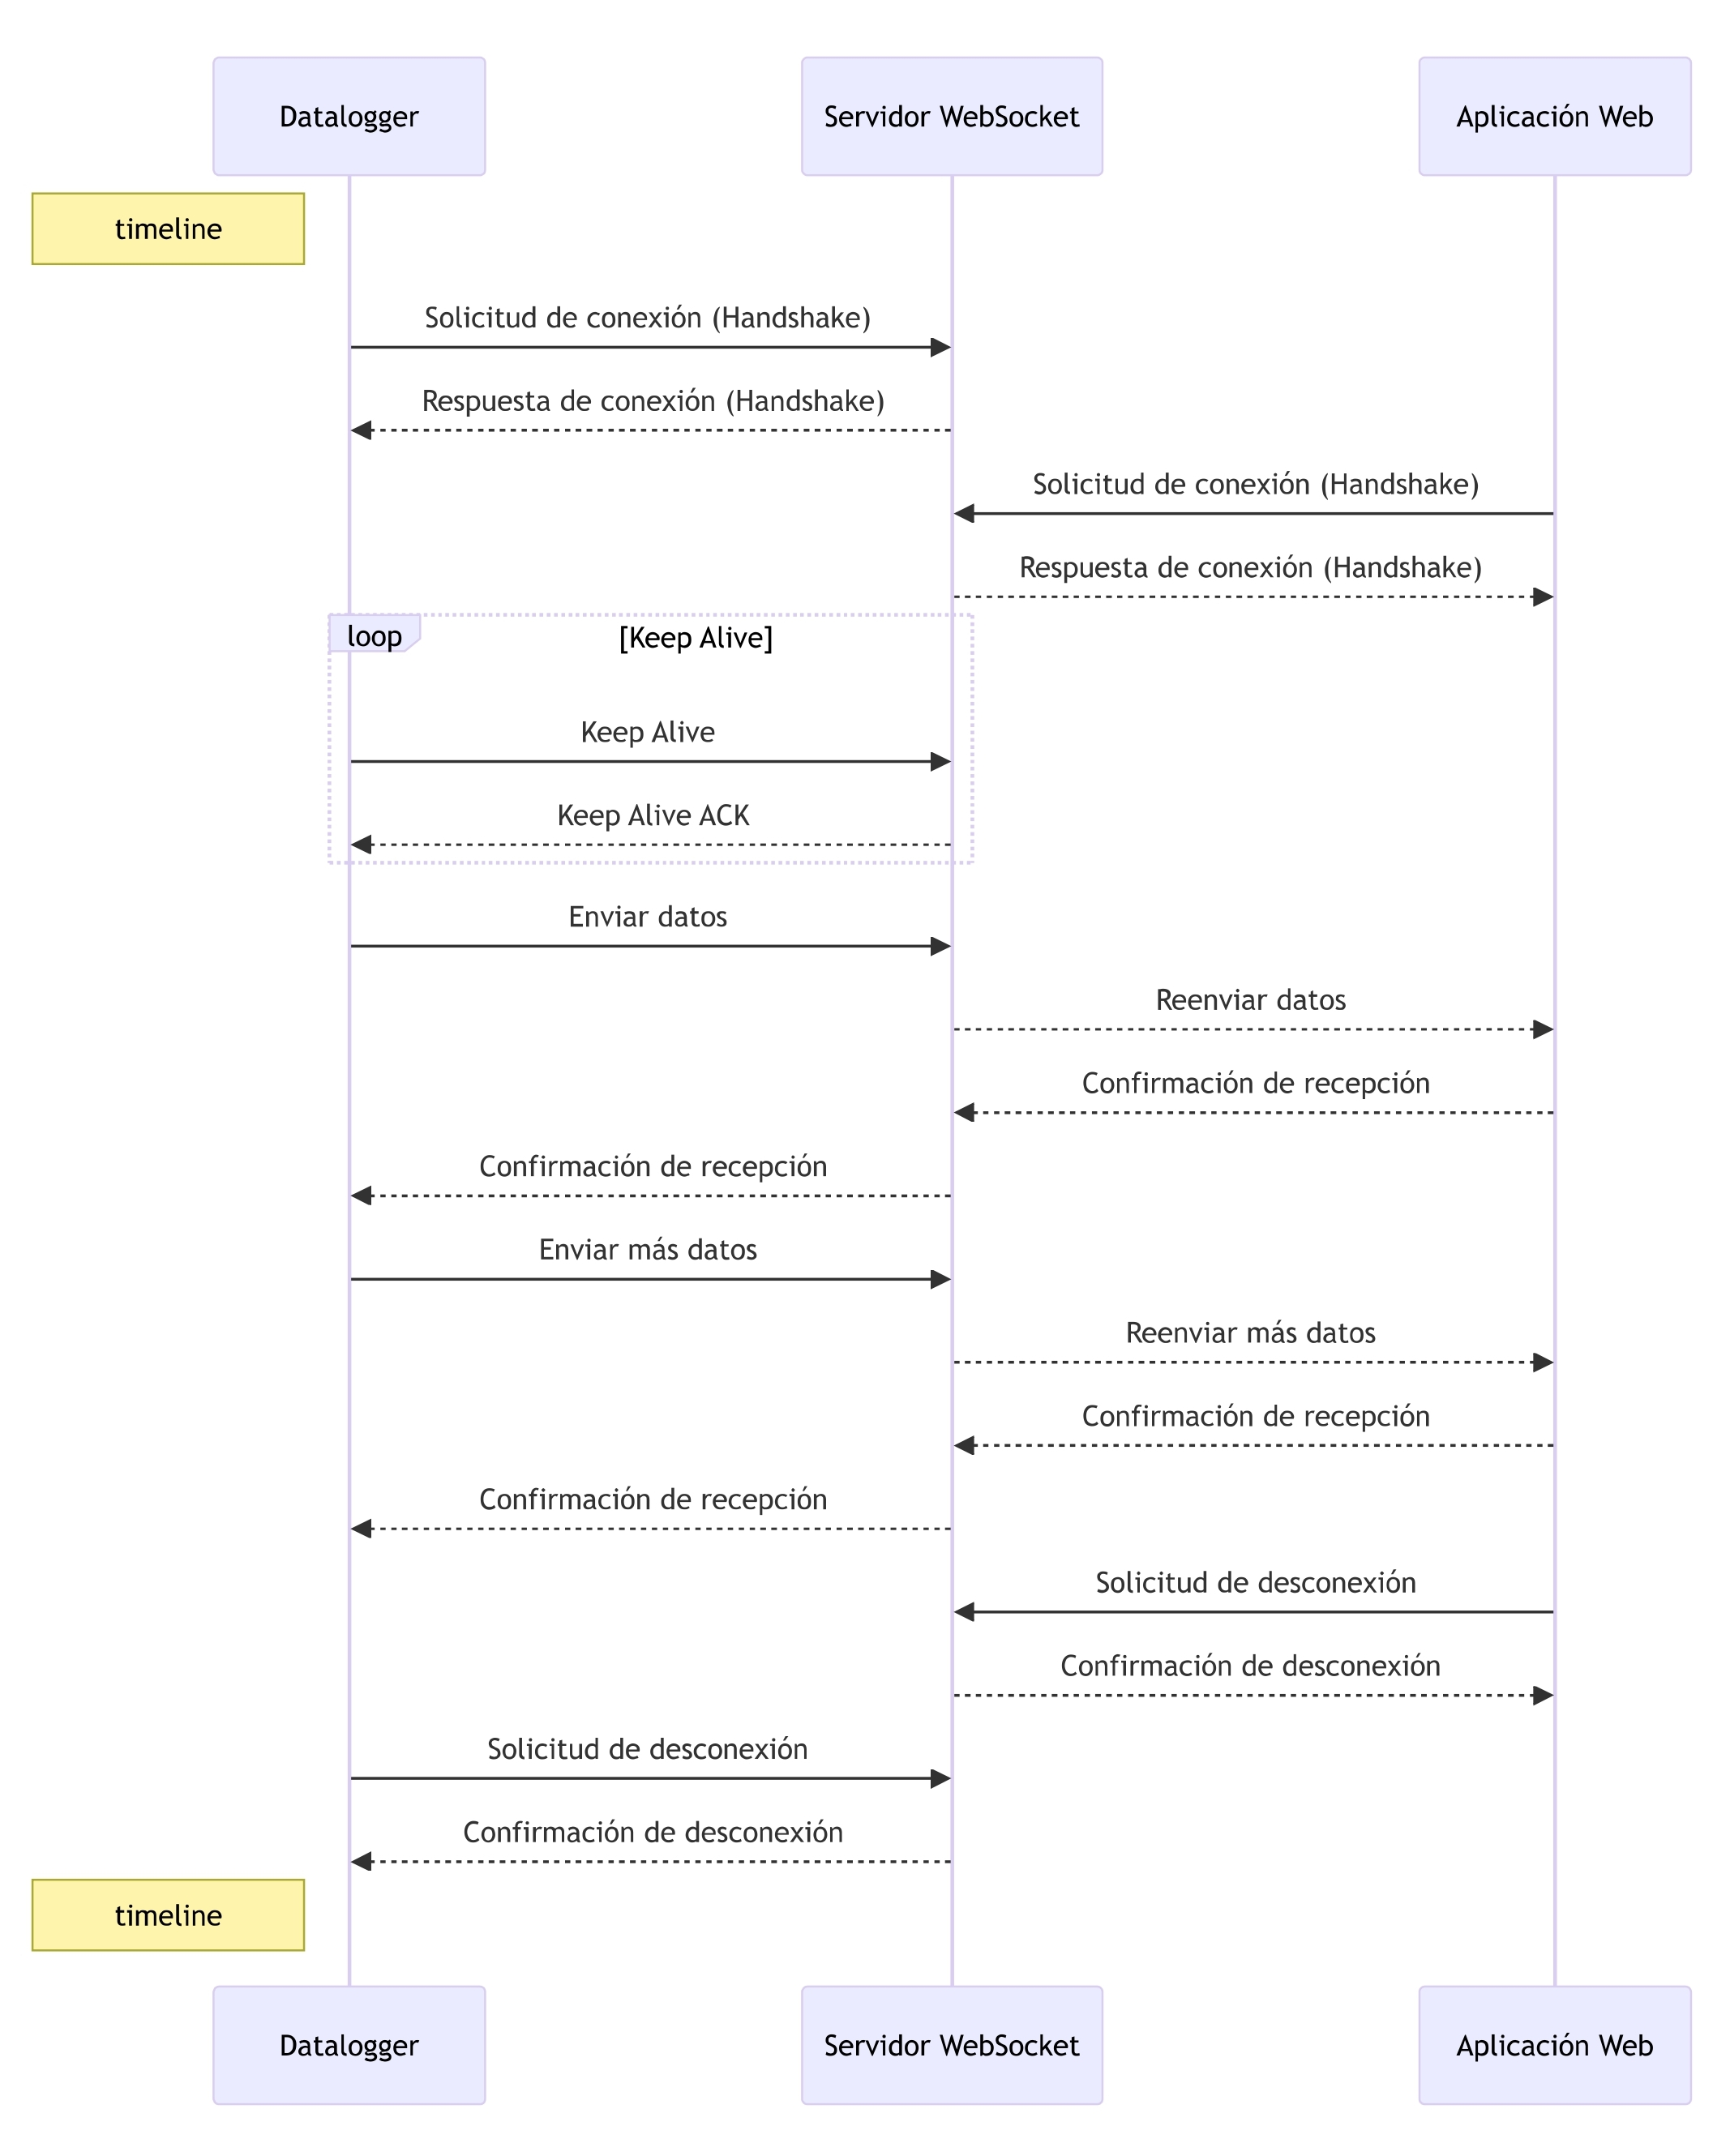
\includegraphics[width=1\linewidth]{Figuras/AplicacionWeb/backend/TimeLineWebSocket.jpg}
    \caption{Diagrama de comunicación entre el servidor \textit{WebSocket}, el cliente de la aplicación web y el \textit{datalogger}.}
    \label{fig:TimeLineWebSocket}
\end{figure}

En la Figura \ref{fig:TimeLineWebSocket} se ilustra la secuencia de interacción entre el \textit{datalogger}, un servidor \textit{WebSocket} y un cliente que utiliza la  aplicación web. Inicialmente, tanto el \textit{datalogger} como la aplicación web realizan una solicitud de conexión al servidor, (\textit{handshake}), la cual es respondida con una confirmación de conexión, estableciendo así el canal de comunicación. El \textit{datalogger} envía periódicamente mensajes de \textit{keep alive} para mantener la conexión activa, a los cuales el servidor responde con una confirmación. Durante la fase de intercambio de datos, el datalogger publica datos al servidor, que posteriormente son reenviados a la aplicación web y se guardan en la base de datos. La aplicación web confirma la recepción de los datos al servidor, y este a su vez confirma dicha recepción al datalogger. Finalmente, cuando se ha terminado de medir todos los valores de velocidad de viento configurados por el operador, ambos clientes envían una solicitud de desconexión al servidor, que responde con una confirmación de desconexión, cerrando así la comunicación. El \textit{datalogger} envía las mediciones de los sensores y la información del controlador en el formato de cadena de caracteres descrito a continuación:

\begin{verbatim}
M;[nro Medición];[fecha];[hora];
[VelPatInst];[VelPatMin];[VelPatMax];[VelPatProm];
[VelIbcInst];[VelIbcMin];[VelIbcMax];[VelIbcProm];
[DirPatInst];[DirPatMin];[DirPatMax];[DirPatProm];
[DirIbcInst];[DirIbcMin];[DirIbcMax];[DirIbcProm];
[BatLevelInst];[BatLevelMin];[BatLevelMax];[BatLevelProm];
[AdcTunelInst];[AdcTunelMin];[AdcTunelMax];[AdcTunelProm];
[PWMLevelInst]
\end{verbatim}

% Para configurar el servidor, se creó el archivo \texttt{routing.py}, el cual define las rutas de los canales, es decir, los puntos de acceso a los consumidores (consumers) que gestionan las conexiones \textit{WebSocket}. La configuración del archivo \texttt{routing.py} se presenta en el Código \ref{cdg:routing}. Cada ruta mapea una URL de \textit{WebSocket} a un consumidor específico. En este caso, \texttt{ChatConsumer} es una clase que maneja las conexiones a la URL \texttt{ws/socket-server/}.



% \begin{lstlisting}[style=pythonstyle, caption={Configuracion del routing para gestionar las conexiones de clientes al servidor \textit{WebSocket}.}, label=cdg:routing,basicstyle=\ttfamily\fontsize{8}{8}\selectfont]
% from django.urls import re_path
% from . import consumers

% websocket_urlpatterns = [
%     re_path(r'ws/socket-server/',consumers.ChatConsumer.as_asgi())
% ]
% \end{lstlisting}

% También se creo el archivo \texttt{consumers.py} define las clases de consumidores que manejan las conexiones \textit{WebSocket}. Un consumidor en Django-channels es una clase que gestiona la conexión con el cliente, incluyendo el manejo de eventos como la recepción y el envío de mensajes. En el codigo \ref{cdg:consumer} se muestra el consumidor implementado

% \begin{lstlisting}[style=pythonstyle, caption={Declaracion de las funciones que utiliza cada consumidor para interactuar con el servidor \textit{WebSocket}.}, label=cdg:consumer,basicstyle=\ttfamily\fontsize{8}{8}\selectfont]
% class ChatConsumer(WebsocketConsumer):
%     def connect(self):
%         self.room_group_name = 'test'
%         async_to_sync(self.channel_layer.group_add)(
%             self.room_group_name,
%             self.channel_name           
%         )
%         self.accept()

%     def disconnect(self, close_code):
%         pass
        
%     def receive(self, text_data):
%         text_data_json = json.loads(text_data)
%         message = text_data_json['message']
%         # message = text_data
%         async_to_sync(self.channel_layer.group_send)(
%             self.room_group_name,
%             {
%                 'type': 'chat_message',
%                 'message': message,
%                 'sender_channel_name': self.channel_name,
%             }
%         )
%         if(len(message)>0):
%             if(message[0] == "M"):
%                 saveMesuareDataBase(message)
%         print('Message:', message)

%     def chat_message(self, event):
%         message = event['message']
%         sender_channel_name = event['sender_channel_name']
%         if sender_channel_name != self.channel_name:
%             self.send(text_data=json.dumps({
%                 'type': 'chat',
%                 'message': message
%             }))
% \end{lstlisting}

% En particular, se implementa la clase \texttt{ChatConsumer}, que hereda de \texttt{WebsocketConsumer}, para gestionar las conexiones \textit{WebSocket}. Esta clase define varios métodos, incluyendo \texttt{connect}, \texttt{disconnect}, \texttt{receive} y \texttt{chat\_message}.

% El método \texttt{connect} se ejecuta cuando un cliente se conecta al servidor \textit{WebSocket}. Dentro de este método, se asigna el nombre del grupo de la sala a \texttt{self.room\_group\_name} y se añade el canal del cliente al grupo utilizando \texttt{async\_to\_sync(self.channel\_layer.group\_add)}. Finalmente, se acepta la conexión mediante \texttt{self.accept()}. Por otro lado, el método \texttt{disconnect} se ejecuta cuando un cliente se desconecta del servidor \textit{WebSocket}.

% (hablar del tipo de string recibido, mejorarlo)
% El método \texttt{receive} recibe y decodifica los mensajes desde JSON para luego enviarlos a un grupo de la sala utilizando \texttt{async\_to\_sync(self.channel\_layer.group\_send)}. Los mensajes que envía el \textit{datalogger} tiene la forma del arreglo declarado en código \ref{cdg:estructuraMensaje}, que contiene toda la información que ha recolectado el \textit{datalogger} en un ciclo de iteración.

El mensaje utiliza el carácter \texttt{;} como separador. La primera letra \texttt{M} es un carácter que el servidor \textit{WebSocket} valida para interpretar que se trata de un mensaje que contiene mediciones y debe ser guardado en la base de datos. A continuación, se incluye el número de medición, la fecha y la hora. Posteriormente, se envían las mediciones de velocidad y dirección de los sensores patrón y bajo calibración. Luego, se envía el nivel de batería de la fuente de alimentación seguido del nivel de tensión del variador del túnel. Todas estas variables se envían en paquetes de cuatro mediciones: el valor instantáneo, el valor mínimo, el valor máximo y el valor promedio. Finalmente, se envía el nivel de PWM que se envía al controlador PID. A continuación, se presenta un ejemplo de mensaje en el que se utiliza una precisión de dos decimales para las mediciones, excepto para el nivel de PWM, que es un valor entero entre 0 y 255.

\begin{verbatim}
    M;634;14-06-2024;16:42:41;
    10.08;10.08;10.08;10.08;
    9.53;9.53;9.53;9.53;
    169;169;169;169;
    175;175;175;175;
    12.02;12.02;12.02;12.02;
    1.25;1.25;1.25;1.25;
    90;
\end{verbatim}

%%%%%%%%%%%%%%%%%%%%%%%%%%%%%%%%%%%%%%%%%%%%%%%%%%%%%%%%%%%%%%%%%%%%%%%%%%%%%%%%%%%%%%%%%%%%%%%%%%%%%%%%%%%%%%%%%%%%%%%%
\subsubsection{Generación de trayectoria y control del túnel}\label{sec:genTrayec}

En la sección \ref{sec:sistemaDeControlPid} se explica cómo funciona el controlador PID del túnel de viento. Este controlador necesita valores de referencia, que se obtienen de un generador de trayectoria diseñado con el método de Paul \cite{RoboFIUBAGenTrayec}. El generador toma de la base de datos los valores de velocidad de viento y tiempos deseados, configurados por el operador en el \textit{front end}, y con estos datos crea una curva de referencia de velocidades de viento en función del tiempo.

\begin{figure}[H]
    \centering
    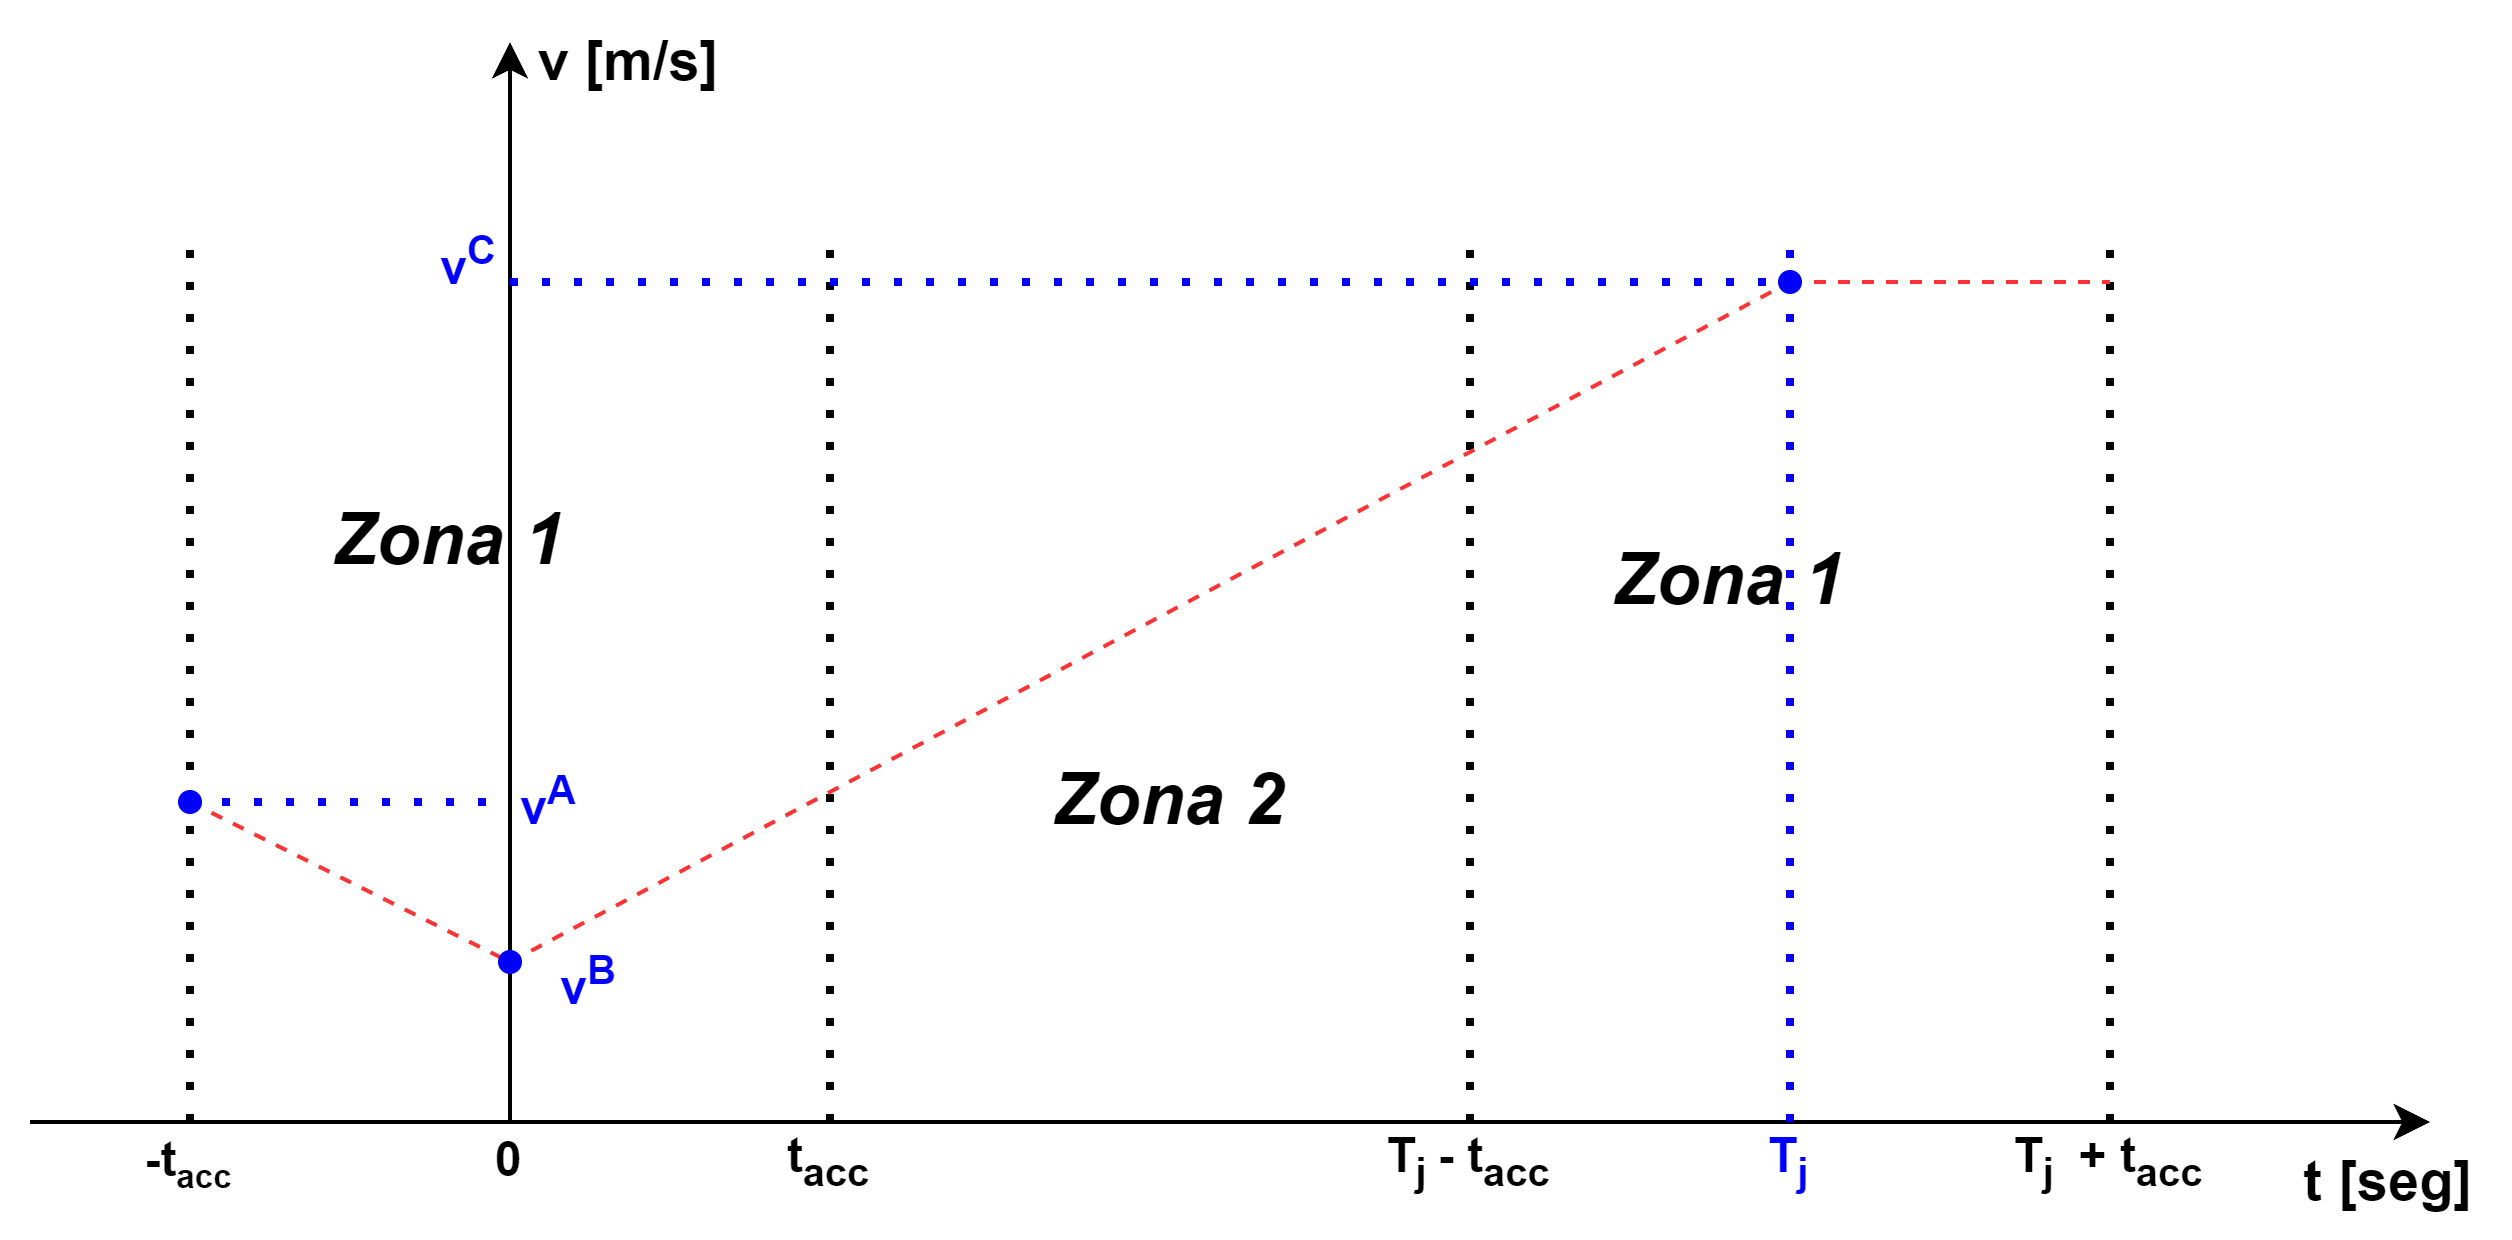
\includegraphics[width=0.9\linewidth]{Figuras/AplicacionWeb/backend/segmentoTrayect.png}
    \caption{Construcción de un segmento para pasar de un valor de velocidad $v^B$ a otro $v^C$ viniendo desde $v^A$.}
    \label{fig:segmentosZona1yZona2}
\end{figure}

El método de Paul consiste en definir, para cada valor de velocidad configurado, dos zonas: una de aceleración constante (zona 1) y otra de velocidad constante (zona 2), como se muestra en la figura \ref{fig:segmentosZona1yZona2}. Cada segmento tiene una duración $T_{j}$ y un tiempo de aceleración $t_{acc}$, de forma tal que no se realicen cambios abruptos en el controlador, permitiendo que los cambios de velocidad del viento sean suaves. Estos cambios suaves se traducen, a través del controlador PID, en cambios suaves en los valores de PWM para el motor. Para construir la zona 2 del segmento $T_{j}$, donde se define $\Delta C = v^C - v^B$, el método de Paul aplica la ecuación \ref{eq:zona2MetodoPaul}:
\begin{equation}
    v(t) = \frac{\Delta C}{T_j} + v^B
    \label{eq:zona2MetodoPaul}
\end{equation}
Para la zona 1 del mismo segmento, donde se define $\Delta A = v^A - v^B$, se aplica la ecuación \ref{eq:zona1MetodoPaul}:
\begin{equation}
    v(t) = \frac{\Delta C}{T_j} \frac{(t + t_{acc})^2}{4t_{acc}} + \frac{\Delta A}{t_{acc}} \frac{(t - t_{acc})^2}{4t_{acc}} + v^B 
    \label{eq:zona1MetodoPaul}
\end{equation}
Combinado estas ecuaciones para todo tiempo $t$ se obtiene un segmento que representa el cambio de velocidad desde $v^A$ hasta $v^c$. Esto garantiza que en la zona 1, donde se realice el enganche de segmento, la aceleración del cambio sea constante, y que en la zona 2, donde se realice la transición de un segmento a otro, la velocidad de cambio sea constante. Se puede revisar en el repositorio \cite{AppGenTrayect} el algoritmo generador de trayectoria. Este se ejecuta en el \textit{back end} y calcula la trayectoria en función de cada segmento, donde se ha configurado un $t_{acc} = \SI{10}{\second}$ y el tiempo de segmento $T_{j}$ se arma en función de los tiempos de crecimiento, estabilización y medición configurados por el operador. 

\begin{figure}[H]
    \centering
    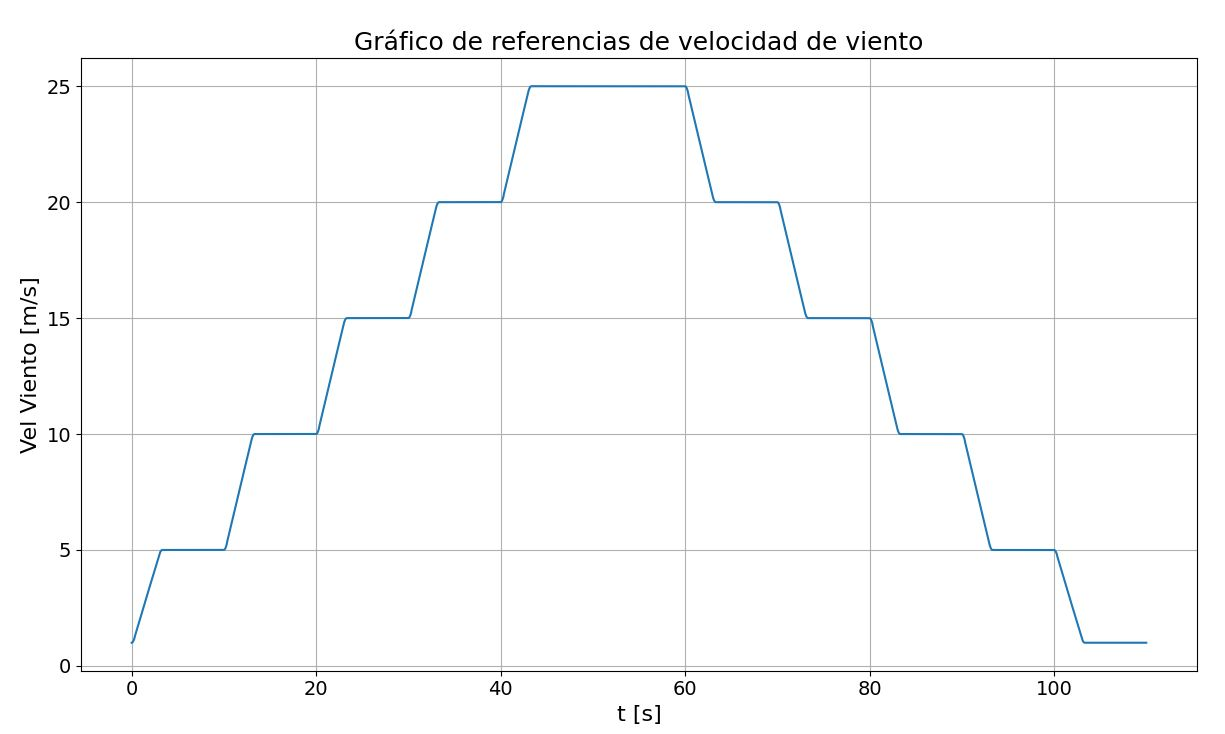
\includegraphics[width=1\linewidth]{Figuras/AplicacionWeb/backend/trayectoriaGenerada.jpg}
    \caption{Trayectoria de referencias de velocidad de viento creada con el método de Paul.}
    \label{fig:trayectoriaGenerada}
\end{figure}

Luego, realiza el encadenamiento de todos esos segmentos dando como resultado un perfil de velocidad de viento como el de la Figura \ref{fig:trayectoriaGenerada}, donde se muestra una trayectoria de ciclo ascendente y descendente para los puntos 5, 10, 15, 20 y 25 \unit{\meter\per\second}, con un tiempo de crecimiento de 2 \unit{\minute}, un tiempo de estabilización de 5 \unit{\minute} y un tiempo de medición de 2 \unit{\minute}. La curva está compuesta en total por diez segmentos, cada uno construido como el de la figura \ref{fig:segmentosZona1yZona2}.
%%%%%%%%%%%%%%%%%%%%%%%%%%%%%%%%%%%%%%%%%%%%%%%%%%%%%%%%%%%%%%%%%%%%%%%%%%%%%%%%%%%%%%%%%%%%%%%%%%%%%%%%%%%%%%%%%%%%%%%%
\subsubsection{Cálculo de incertidumbre}\label{sec:calculoIncertidumbre}

El proceso de calcular la incertidumbre expandida para todos los puntos de viento medidos se realiza (basado en la norma \cite{GUM}) según el algoritmo del diagrama de flujo de la figura \ref{fig:DiagramaFlujoCalculoIncertidumbre}.

\begin{figure}[H]
    \centering
    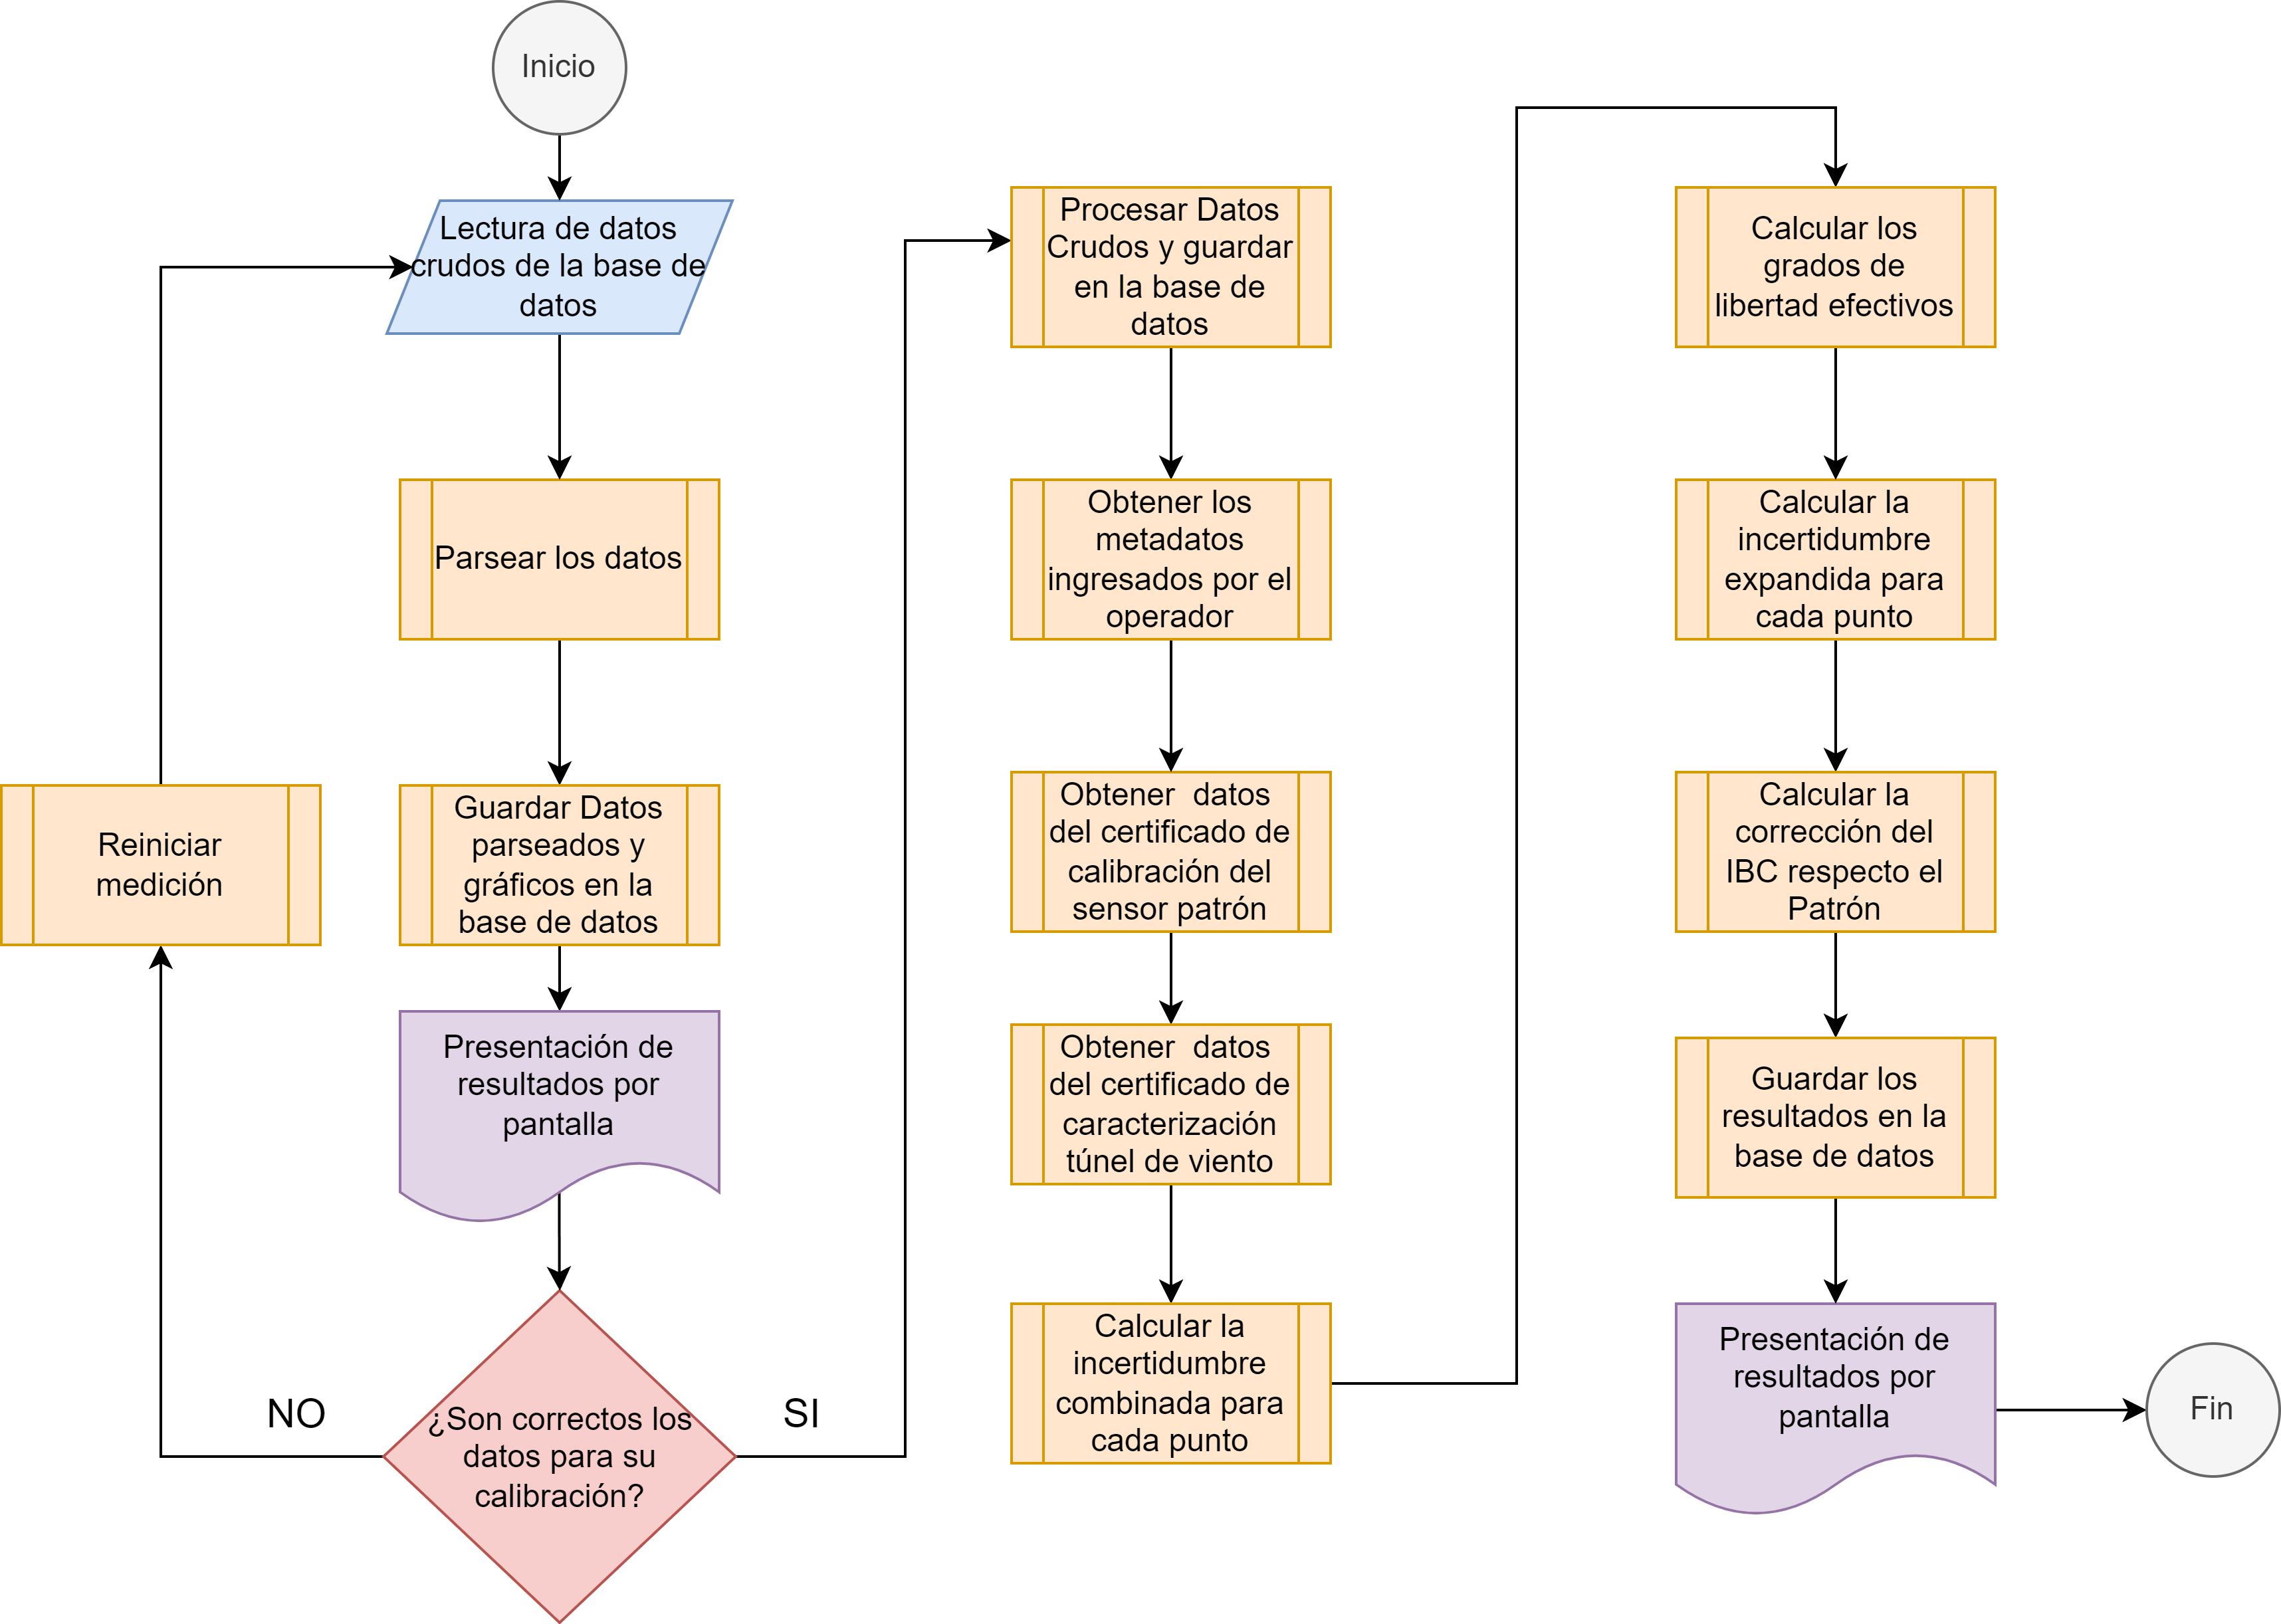
\includegraphics[width=1\linewidth]{Figuras/AplicacionWeb/backend/DiagramaFlujoCalculoIncertidumbre.png}
    \caption{Diagrama de flujo del para el calculo de incertidumbre expandida.}
    \label{fig:DiagramaFlujoCalculoIncertidumbre}
\end{figure}

Después de completar los ciclos de medición ascendente y descendente, se dispone de un conjunto de muestras de velocidad y dirección del viento. El algoritmo lee estos datos y extrae la parte plana y estable de las mediciones (como se ilustra en la Figura \ref{fig:curvaEscalon} de la sección siguiente). Este procedimiento se aplica a cada segmento y se denomina \texttt{parseo de datos}. Posteriormente, se muestran los datos crudos extraídos en pantalla, donde el operador, desde el \textit{front end}, puede iniciar el cálculo de incertidumbre, siempre que considere que las muestras son útiles. En caso contrario, puede reiniciar las mediciones y obtener un nuevo perfil. Si los datos son correctos para la calibración, se calcula el promedio $\bar{v}$ y el desvío estándar $\sigma_{v}$ de las mediciones extraídas. A continuación, para cada valor de viento promedio obtenido, se elabora el presupuesto de incertidumbre, obteniendo los datos de histéresis del patrón y del IBC a partir de la diferencia de los valores promedio del ciclo ascendente menos el ciclo descendente. Luego, se procede con la lectura de los metadatos ingresados por el operador, específicamente la resolución de los instrumentos y el área de bloqueo de los anemómetros, donde este último se utiliza para el cálculo del factor de bloqueo, según la ecuación \ref{eq:FactorDeBloqueo}, donde $S_{T}$ corresponde al área transversal de la zona de medición del túnel de viento y $S_{A}$ se corresponde al área efectiva de bloqueo del sensor y su soporte. Este valor se utiliza para corregir las mediciones del IBC y del patrón, y se agrega al presupuesto su respectiva incertidumbre según la ecuación \ref{eq:incertiFactorBloqueo}.


\begin{equation}
    \centering
    F_{bk}= \frac{S_{A} }{S_{T}}
    \label{eq:FactorDeBloqueo}
\end{equation}

\begin{equation}
    \centering
    \Delta F_{bk} =  \sqrt{\left\lvert \frac{\partial F}{\partial S_T} \right\rvert^2 \left\lvert\Delta S_T\right\rvert^2 + \left\lvert \frac{\partial F}{\partial S_A} \right\rvert^2 \left\lvert\Delta S_A\right\rvert^2} = \left( \frac{-S_{A}}{S_{T}^{2}} \right)^2 (\Delta S_T)^2 + \left( \frac{1}{S_{T}} \right)^2 (\Delta S_A)^2
    \label{eq:incertiFactorBloqueo}
\end{equation}
A continuación, el algoritmo obtiene los datos de calibración del sensor patrón a partir de una regresión lineal de los puntos discretos del certificado. En esa curva obtenida, se evalúa los valores promedio del patrón $\bar{v}_{Pat}$. Esto se hace así porque no siempre el patrón está calibrado en los mismos puntos en los que se lo va a utilizar. Lo mismo se realiza con el certificado del túnel, se extrae los valores de estabilidad, homogeneidad y el factor de calibración del túnel para los valores promedio del IBC $\bar{v}_{IBC}$. Con todas estas incertidumbres normalizadas y multiplicadas por su coeficiente de sensibilidad $c_{i}$, se obtiene la incertidumbre estándar. Luego, se realiza la suma de los cuadrados, ecuación \ref{eq:incertCombinadaSoft}, de cada incertidumbre estándar y se aplica la raíz cuadrada para obtener la incertidumbre combinada para cada punto configurado por el operador.
\begin{equation}
    \centering
    u_c = \sqrt{\sum_{i=1}^{n} (u_{i} \cdot c_{i})^2}.
\label{eq:incertCombinadaSoft}
\end{equation}

En base al número de mediciones, se calculan los grados de libertad efectivos y con este número, solicitando un intervalo de confianza del 95\%, se evalúa la distribución $t$ de Student para obtener el factor de cobertura $k$. Luego, se multiplica este número por cada incertidumbre combinada correspondiente para obtener la incertidumbre expandida 
\begin{equation}
    \centering
    U = k \cdot u_c.
\label{eq:incertExpandidaSoft}
\end{equation}

Finalmente, se presentan en pantalla un resumen de todos los resultados, además de disponer de botones para descargar los gráficos y tablas correspondientes a los datos crudos, la histéresis y los resultados de calibración.

% Luego, se grafica la curva de histéresis, como se muestra en la figura \ref{fig:CurvaHisteresis}, junto con una tabla para analizar la alinealidad del IBC (figura \ref{fig:TablaAlinealidad}). Además, se presenta la curva de calibración con sus correspondientes incertidumbres expandidas tanto para los datos del ciclo ascendente como del descendente (figura \ref{fig:CurvaCalibracion}). Finalmente, se incluye una tabla (figura \ref{fig:TablaIncertidumbres}) donde se especifican la incertidumbre combinada, la incertidumbre expandida, la corrección y los grados de libertad para cada punto donde se realizó la calibración del anemómetro.

%%%%%%%%%%%%%%%%%%%%%%%%%%%%%%%%%%%%%%%%%%%%%%%%%%%%%%%%%%%%%%%%%%%%%%%%%%%%%%%%%%%%%%%%%%%%%%%%%%%%%%%%%%%%%%%%%%%%%%%%
\subsection{Front End}\label{sec:frontEnd}

El front end se encarga de gestionar la interacción del usuario mediante formularios, botones y eventos. Además, facilita la comunicación con el \textit{back end} utilizando Django y \textit{WebSockets}. Por último, se encarga de la presentación de tablas y gráficos al usuario, optimizando la experiencia de usuario (UI/UX). La aplicación web presenta una plantilla de inicio, como se muestra en la figura \ref{fig:index}. En la cabecera se visualiza, el logotipo correspondiente al SMN, el nombre del sistema definido como \textbf{Eclipse 1.0}, y el nombre y tipo de perfil de usuario. En el lado izquierdo, se encuentran cuatro botones: \textbf{Temperatura y humedad}, \textbf{Temperatura}, \textbf{Presión} y \textbf{Viento}, cada uno con su respectiva descripción. Se ha realizado este diseño ya que a futuro se va a escalar el software para incluir las otras magnitudes con las que trabaja el laboratorio del SMN. En el pie de página, se presentan los enlaces a las herramientas utilizadas en el desarrollo del proyecto.
\begin{figure}[H]
    \centering
    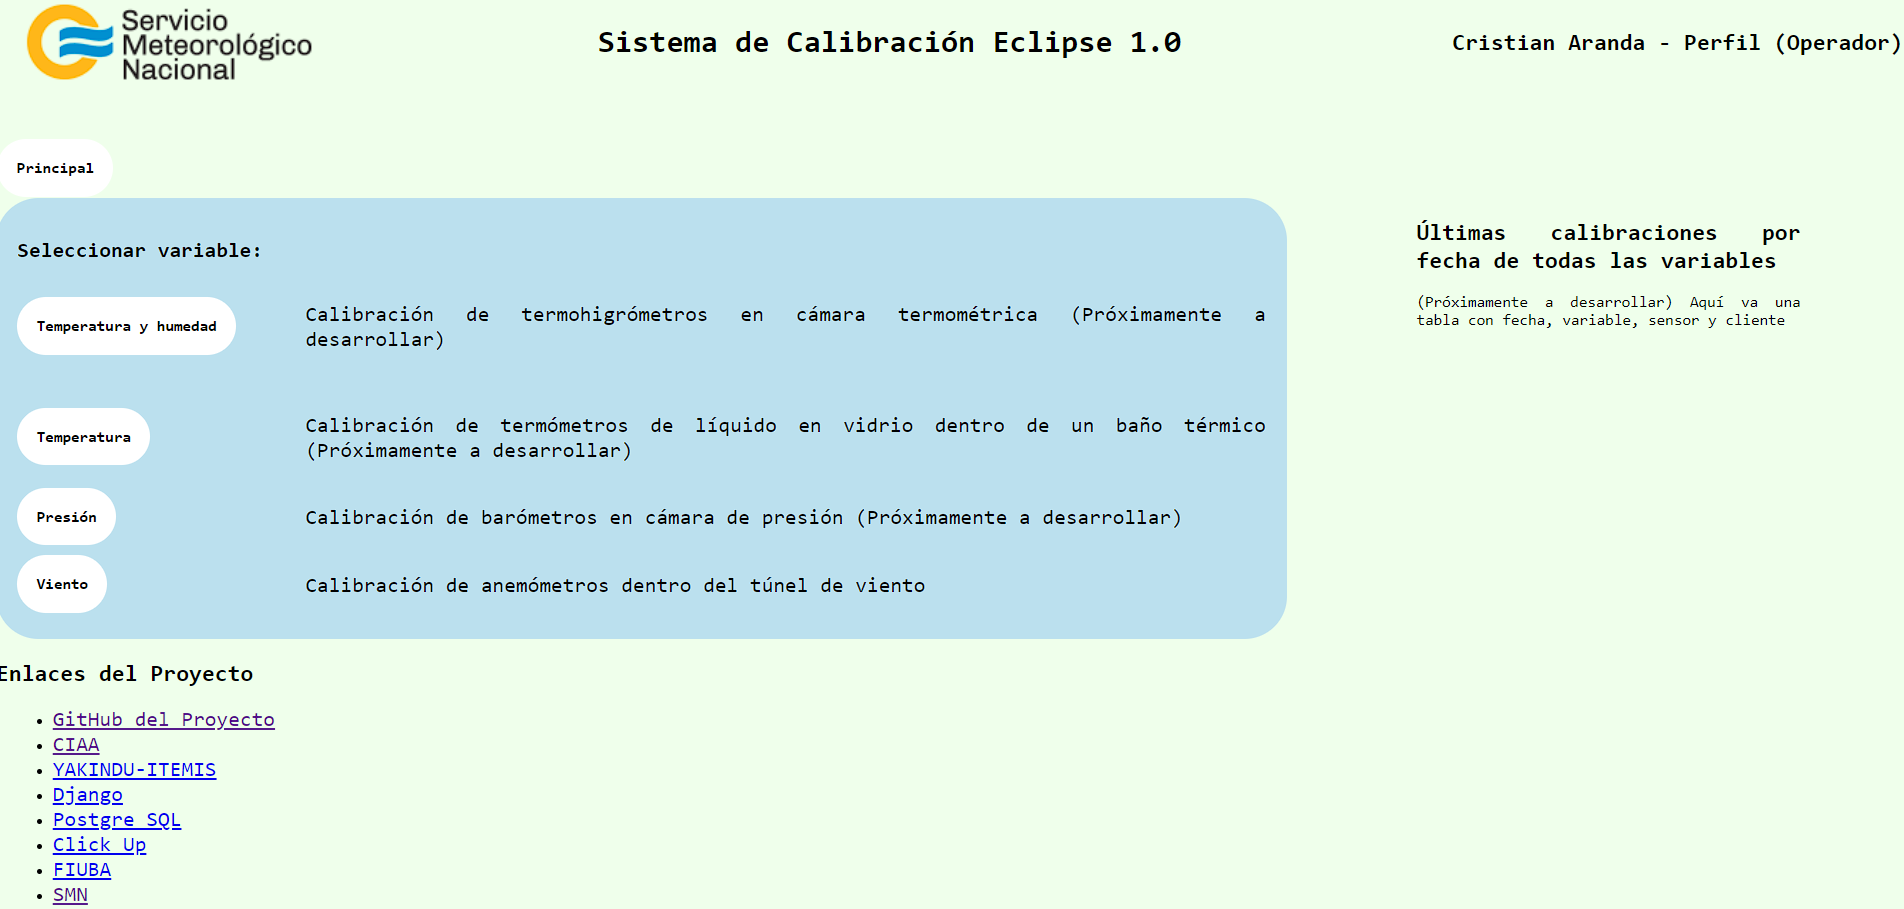
\includegraphics[width=1\linewidth]{Figuras/AplicacionWeb/frontend/index.png}
    \caption{Pantalla de inicio de la aplicación web.}
    \label{fig:index}
\end{figure}
El usuario hace click en el botón \textbf{Viento} y se activa la vista de la Figura \ref{fig:iniciarCalibViento}, donde le consulta al usuario, si desea iniciar o no una calibración de anemómetros.
\begin{figure}[H]
    \centering
    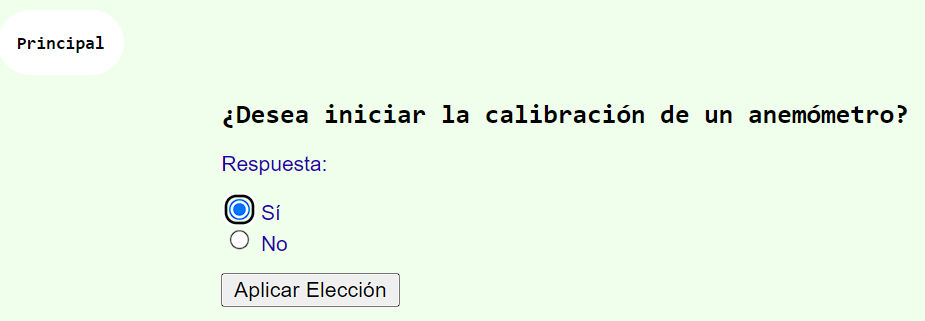
\includegraphics[width=0.7\linewidth]{Figuras/AplicacionWeb/frontend/iniciarCalibViento.png}
    \caption{Vista para confirmar si se desea realizar o no una calibración.}
    \label{fig:iniciarCalibViento}
\end{figure}
Si el usuario responde afirmativamente, se abre a izquierda una barra de navegación, como se muestra en la figura \ref{fig:barraNavegIzq}, que permite navegar por la aplicación web. En el cuerpo de la aplicación se presenta una serie de formularios y botones para cargar los metadatos, configurar los equipos, iniciar las mediciones y, finalmente, procesar y presentar los resultados. Además, el usuario puede utilizar el botón \textbf{Salir}, que lo redirige a la pestaña de inicio.

\begin{figure}[H]
    \centering
    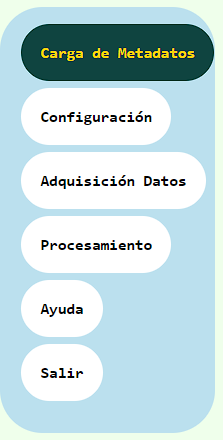
\includegraphics[width=0.2\linewidth]{Figuras/AplicacionWeb/frontend/barraNavegIzq.png}
    \caption{Barra lateral izquierda de navegación.}
    \label{fig:barraNavegIzq}
\end{figure}
%%%%%%%%%%%%%%%%%%%%%%%%%%%%%%%%%%%%%%%%%%%%%%%%%%%%%%%%%%%%%%%%%%%%%%%%%%%%%%%%%%%%%%%%%%%%%%%%%%%%%%%%%%%%%%%%%%%%%%%%
\subsubsection{Carga de metadatos}\label{sec:cargaMetadatos}

El contenido principal de la primera vista, llamada \textbf{Carga de Metadatos}, se muestra en la Figura \ref{fig:cargaMetadata}. En esta vista, se deben ingresar la marca, el modelo, el número de serie, el número de patrimonio (identificador de instrumentos del SMN), la resolución y el área de bloqueo del instrumento medido previamente con una cinta métrica, tanto del sensor patrón como del sensor bajo calibración. Luego, se debe cargar la información del certificado de calibración del instrumento patrón utilizado, incluyendo la fecha de generación, los puntos en los que fue calibrado, los valores obtenidos por cada punto, las correcciones obtenidas y su respectiva incertidumbre. Por último, se deben ingresar los datos del certificado de caracterización del túnel de viento, especificando la fecha de emisión, los puntos medidos en el ensayo, los valores de estabilidad y de homogeneidad del flujo de aire en la zona de medición. Además, se debe agregar el factor de calibración definido en la tabla \ref{tab:fuenteIncert}. Una vez cargada toda la información, el operador debe presionar el botón \textbf{Cargar}, o si desea borrar toda la información del formulario, debe presionar \textbf{Limpiar campos}. Parte de esta información luego será utilizada para el cálculo de la incertidumbre expandida del sensor bajo calibración y toda esta información ingresada por el usuario se guardan en la base de datos.

\begin{figure}[H]
    \centering
    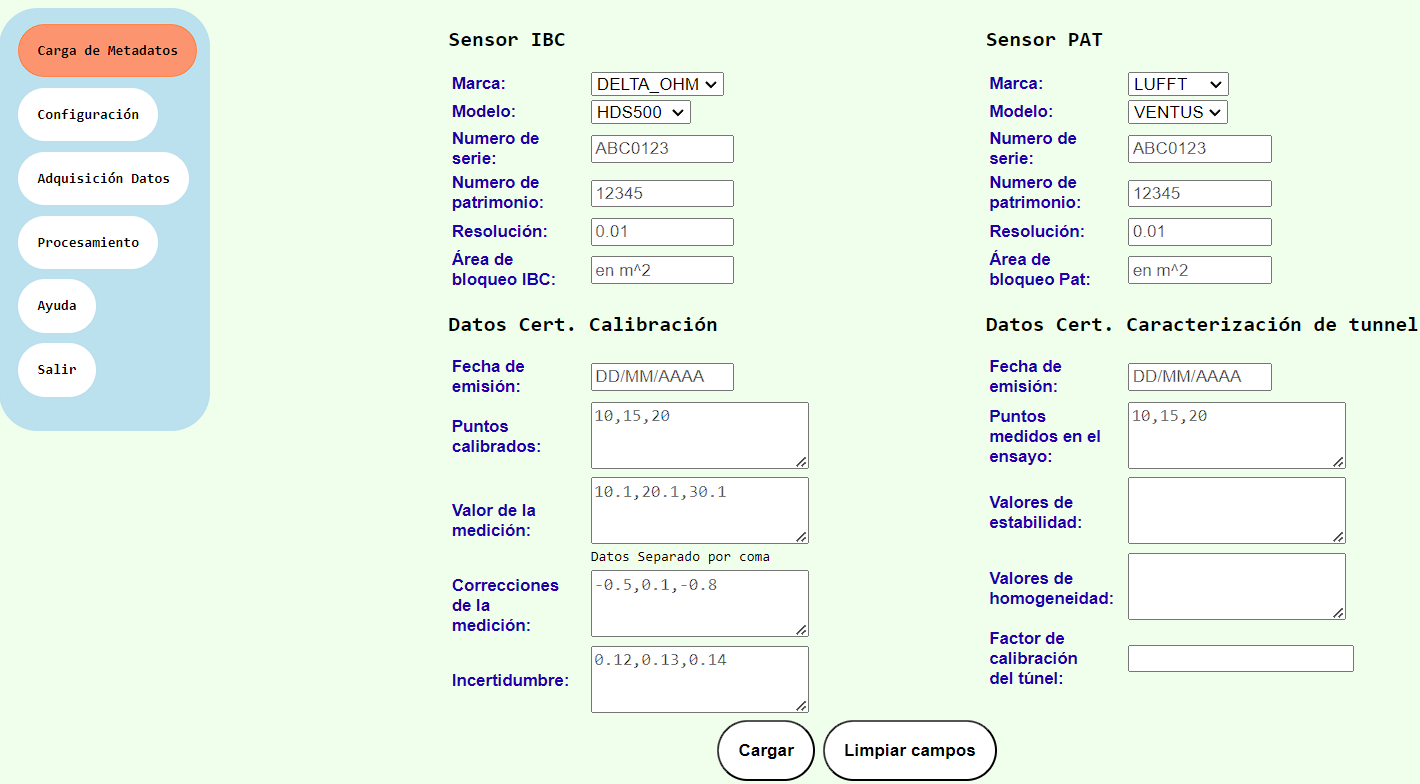
\includegraphics[width=1\linewidth]{Figuras/AplicacionWeb/frontend/cargaMetadata.png}
    \caption{Vista para cargar los metadatos de la calibración.}
    \label{fig:cargaMetadata}
\end{figure}

%%%%%%%%%%%%%%%%%%%%%%%%%%%%%%%%%%%%%%%%%%%%%%%%%%%%%%%%%%%%%%%%%%%%%%%%%%%%%%%%%%%%%%%%%%%%%%%%%%%%%%%%%%%%%%%%%%%%%%%%
\subsubsection{Configuración}\label{sec:configSistema}

El contenido principal de la segunda vista, denominada \textbf{Configuración}, se muestra en la Figura \ref{fig:configEquipos}. En esta vista, a la izquierda, se configura el \textit{datalogger} diseñado en el capítulo \ref{cap:datalogger}. Se pueden seleccionar la marca, el modelo y el número de serie del \textit{datalogger}. Posteriormente, se especifica el tiempo de muestreo y el tiempo de tabla, se configuran los puertos de comunicación serie del \textit{datalogger}, los LEDs de recepción y la velocidad en baudios para cada anemómetro.

\begin{figure}[H]
    \centering
    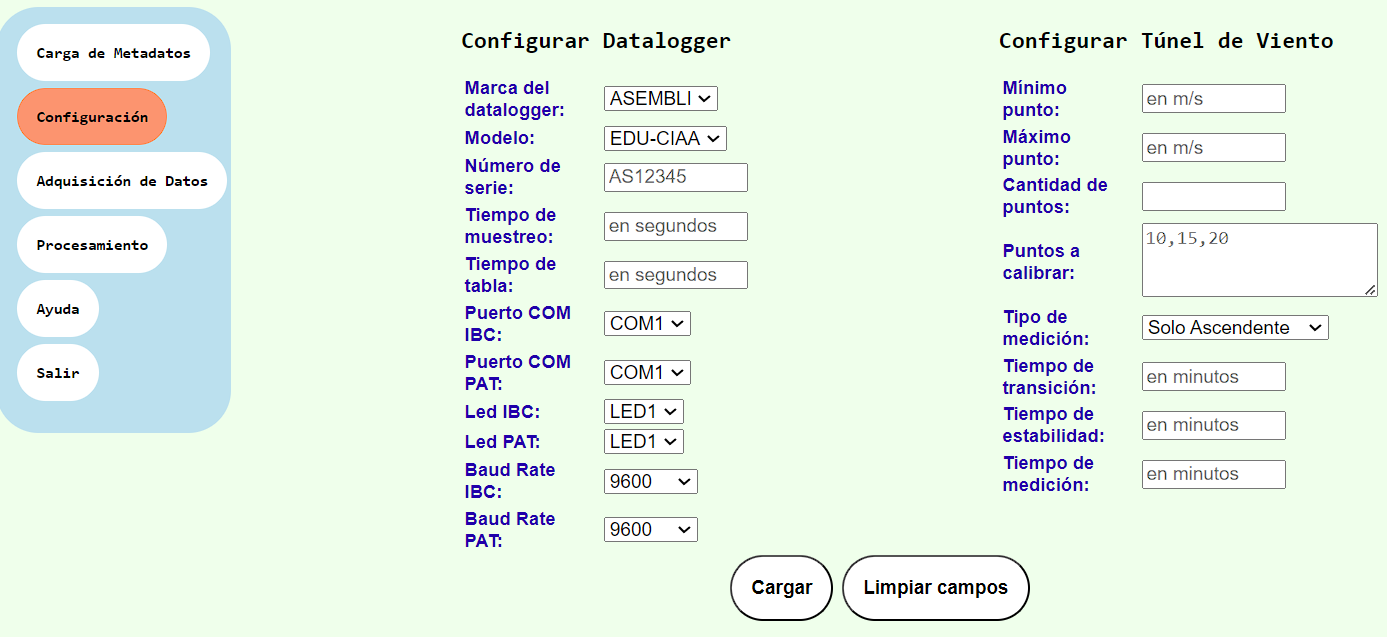
\includegraphics[width=1\linewidth]{Figuras/AplicacionWeb/frontend/configEquipos.png}
    \caption{Vista para configurar los equipos involucrados en la calibración.}
    \label{fig:configEquipos}
\end{figure}

A la derecha, se configura el túnel de viento. Aquí se establecen los puntos mínimo y máximo de velocidad, la cantidad de puntos donde se desea medir, los valores de velocidad en metros por segundo, y el tipo de perfil de medición, que puede ser ascendente, descendente o ambos. También se configuran los tiempos de transición, de estabilidad y de medición para cada punto, necesarios para generar el perfil de trayectoria explicado en la sección \ref{sec:genTrayec}. Estos tiempos se ilustran sobre el escalón de la Figura \ref{fig:curvaEscalon}.

\begin{figure}[H]
    \centering
    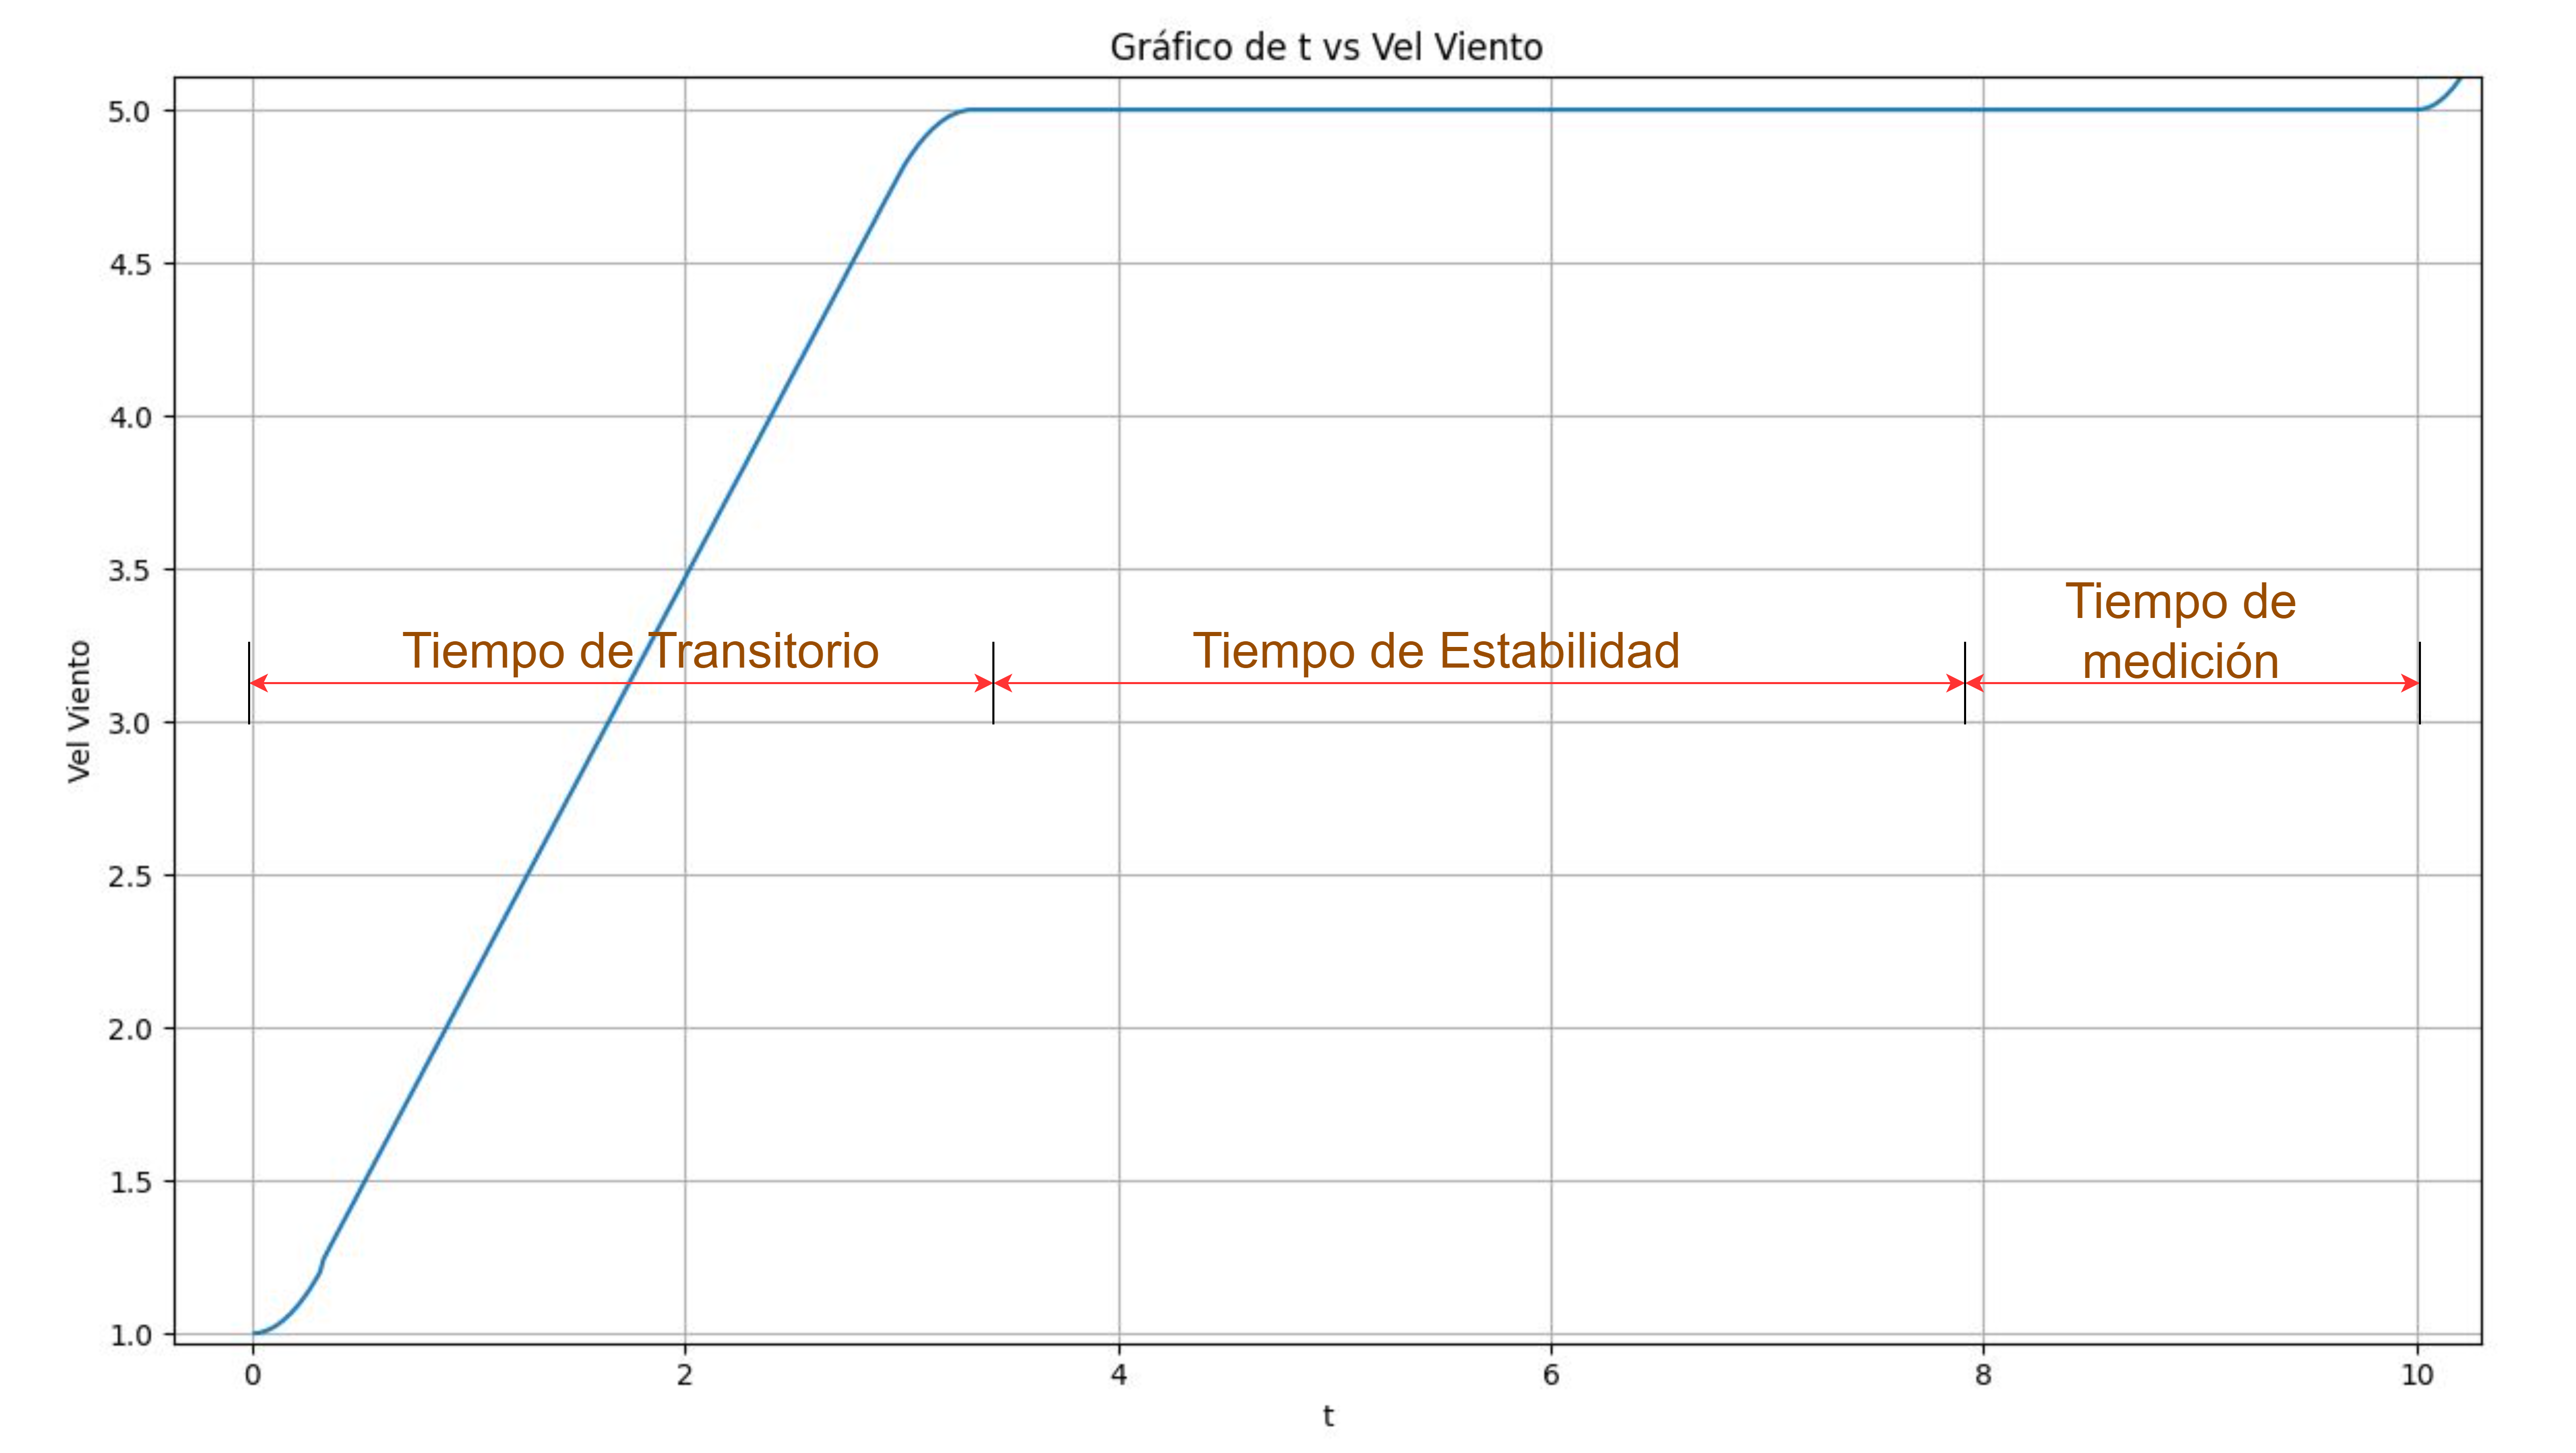
\includegraphics[width=0.9\linewidth]{Figuras/AplicacionWeb/frontend/curvaEscalon.png}
    \caption{Configuración de tiempos para el generador de trayectoria en $\SI{5}{\meter\per\second}$.}
    \label{fig:curvaEscalon}
\end{figure}

Una vez que los datos de configuración están cargados, el usuario puede hacer clic en el botón \textbf{Cargar} para subirlos a la base de datos o en \textbf{Limpiar campos} para borrar los campos de esta vista.


%%%%%%%%%%%%%%%%%%%%%%%%%%%%%%%%%%%%%%%%%%%%%%%%%%%%%%%%%%%%%%%%%%%%%%%%%%%%%%%%%%%%%%%%%%%%%%%%%%%%%%%%%%%%%%%%%%%%%%%%
\subsubsection{Adquisición de datos}\label{sec:adquisicionDatos}

Una vez cargados todos los datos, el software muestra la vista de la Figura \ref{fig:adquisicionDatos}. Al hacer clic en el botón \textbf{Iniciar Medición}, se envían todas las configuraciones al \textit{datalogger} a través del servidor \textit{WebSocket} mediante comandos detallados en la Tabla \ref{tab:comandoDataloggerWeb}. Luego, se activa un temporizador que multiplica el tiempo de un escalón, como el de la Figura \ref{fig:curvaEscalon}, por la cantidad de puntos ingresados e indica el tiempo restante para que termine todas las mediciones. El software también envía, a intervalos de un segundo, un valor de referencia del generador de trayectoria al \textit{datalogger} para que éste genere un nivel de PWM y lo envíe al variador de velocidad del motor. Al mismo tiempo, se reciben las mediciones del sensor patrón e IBC, y se va construyendo el perfil de mediciones, con la dirección del viento a la izquierda y la intensidad a la derecha.

\begin{figure}[H]
    \centering
    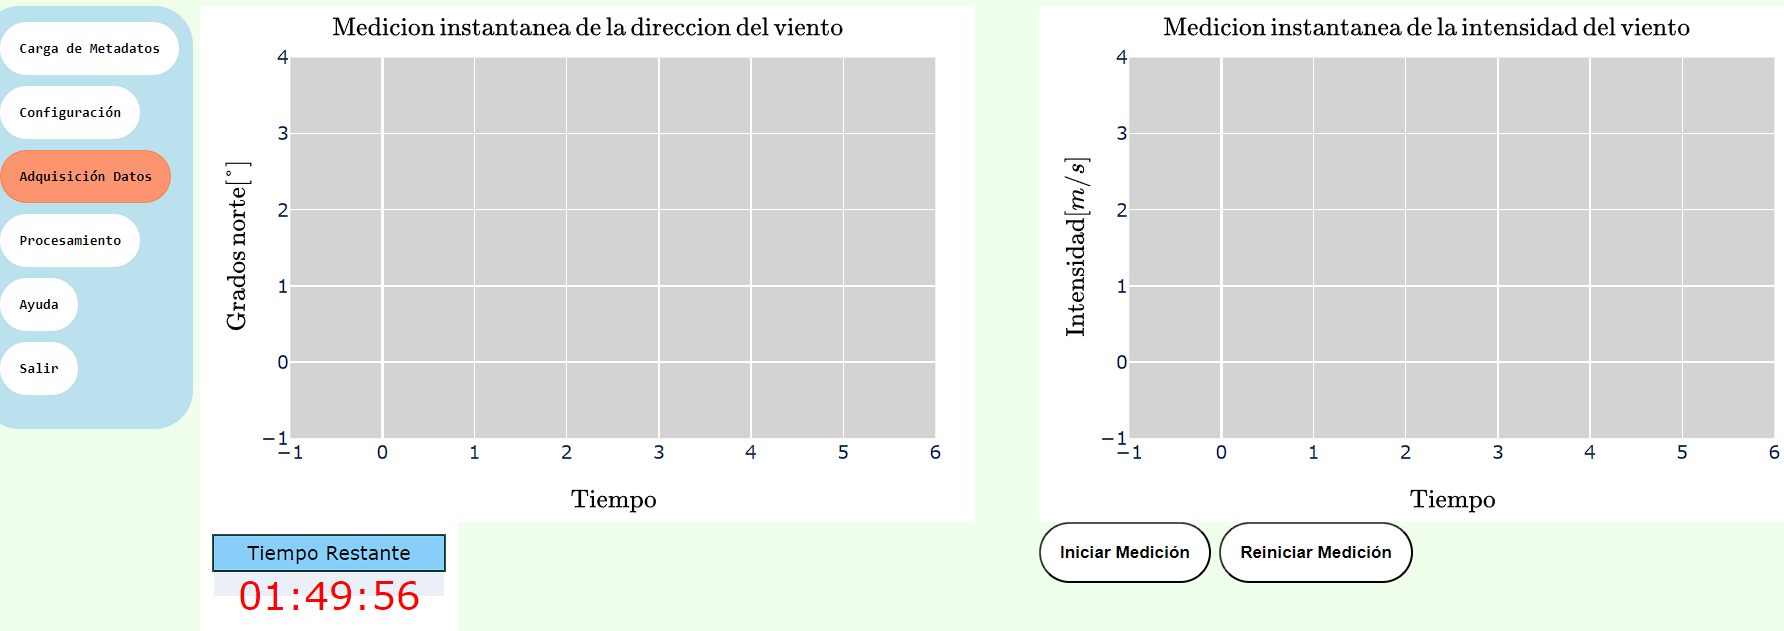
\includegraphics[width=1\linewidth]{Figuras/AplicacionWeb/frontend/adquisicionDatos.png}
    \caption{Vista de la adquisición de datos.}
    \label{fig:adquisicionDatos}
\end{figure}

En caso de que el operador precise reiniciar las mediciones puede activar el botón \textbf{Reiniciar Medición}, el cual genera la vista de la figura \ref{fig:borrarMediciones}, que informa que si reinicia se borraran las mediciones ya adquiridas.

\begin{figure}[H]
    \centering
    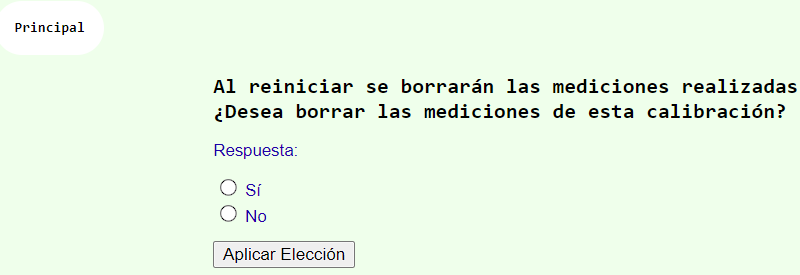
\includegraphics[width=0.8\linewidth]{Figuras/AplicacionWeb/frontend/borrarMediciones.png}
    \caption{Vista para confirmar si se desea borrar o no los datos crudos de una calibración.}
    \label{fig:borrarMediciones}
\end{figure}



%%%%%%%%%%%%%%%%%%%%%%%%%%%%%%%%%%%%%%%%%%%%%%%%%%%%%%%%%%%%%%%%%%%%%%%%%%%%%%%%%%%%%%%%%%%%%%%%%%%%%%%%%%%%%%%%%%%%%%%%
\subsubsection{Procesamiento}\label{sec:ProcesamientoDatos}
Luego de que se acabe el tiempo del temporizador, el software redirige a la vista \textbf{Procesamiento} que se muestra en la Figura \ref{fig:procesarDatos1}. En esta vista, se grafican las curvas ascendente y descendente de las velocidades de viento del sensor patron y bajo calibración. En el título del gráfico se indica la magnitud, el número de serie y patrimonio del sensor bajo calibración. Toda la información y datos se leen desde la base de datos, ya que se fueron almacenando en la misma a medida que ingresaron. Además, cada gráfico cuenta con un botón para ser descargado.

\begin{figure}[H]
    \centering
    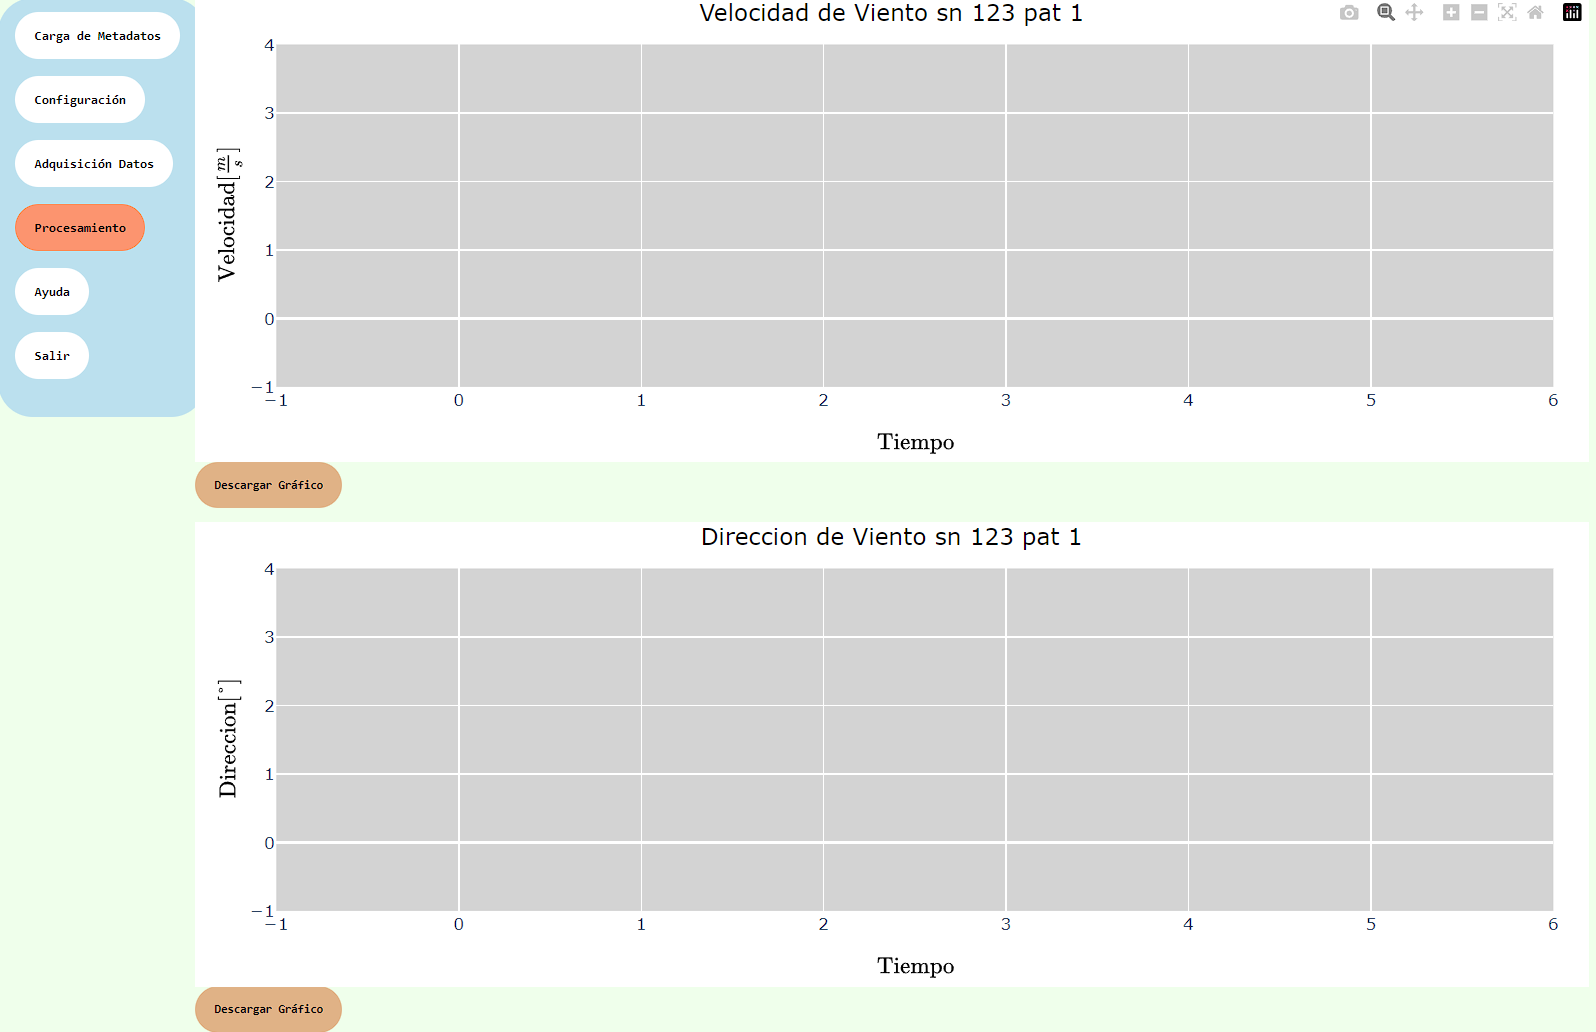
\includegraphics[width=1\linewidth]{Figuras/AplicacionWeb/frontend/procesarDatos1.png}
    \caption{Vista para el procesamiento de datos y visualización de gráficos.}
    \label{fig:procesarDatos1}
\end{figure}

En la parte inferior de la vista, como se ve en la figura \ref{fig:procesarDatos2} se muestran tablas con los datos parseados, que corresponden a la extracción de los datos de la parte plana, equivalente al tiempo de medición, como por ejemplo en el gráfico de la Figura \ref{fig:curvaEscalon} se tiene alrededor de 120 muestras en $\SI{5}{\meter\per\second}$. El operador revisa estos datos y, si están dentro del entorno del punto de medición configurado, debe presionar el botón \textbf{Calcular Incertidumbre}. En caso contrario, puede reiniciar las mediciones, lo que lo devolverá a la vista de adquisición de datos. De igual forma cada tabla cuenta con un botón para ser descargado en formato $.csv$

\begin{figure}[H]
    \centering
    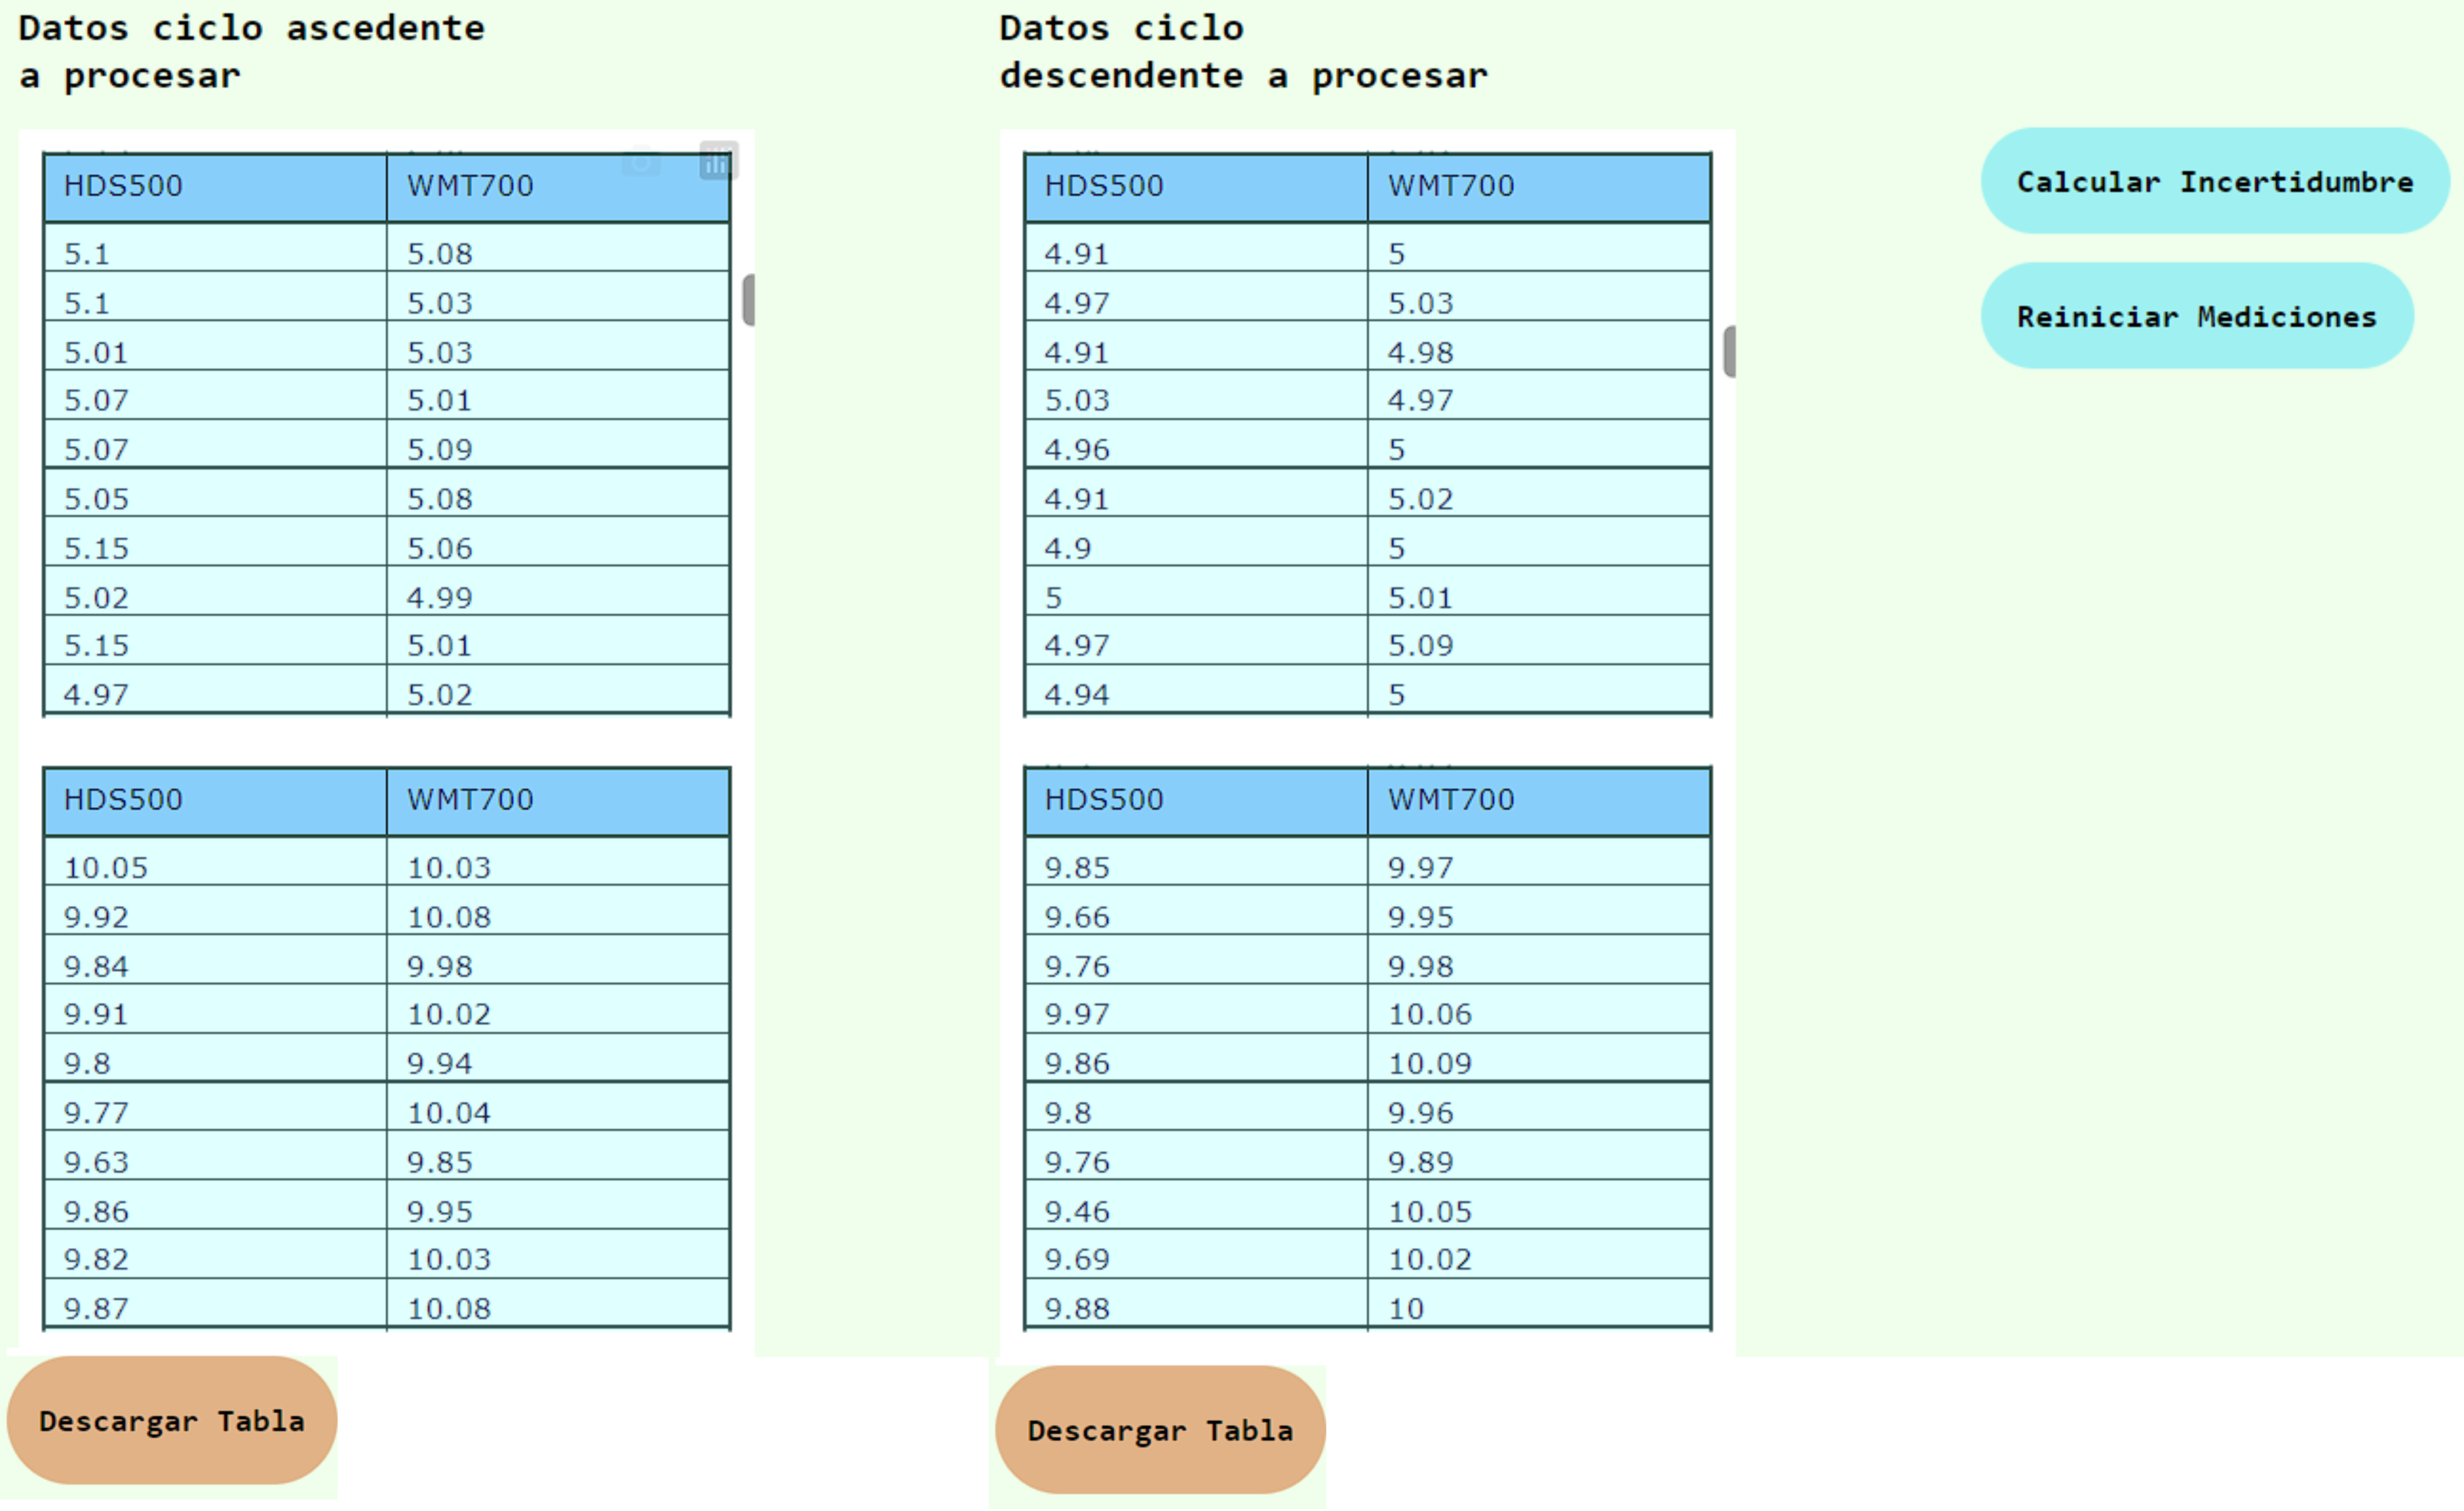
\includegraphics[width=0.9\linewidth]{Figuras/AplicacionWeb/frontend/procesarDatos2.png}
    \caption{Vista para la revisión de datos parseados y cálculo de incertidumbre.}
    \label{fig:procesarDatos2}
\end{figure}



%%%%%%%%%%%%%%%%%%%%%%%%%%%%%%%%%%%%%%%%%%%%%%%%%%%%%%%%%%%%%%%%%%%%%%%%%%%%%%%%%%%%%%%%%%%%%%%%%%%%%%%%%%%%%%%%%%%%%%%%
\subsubsection{Resumen del presupuesto}\label{sec:Resultados}

Cuando se hace clic en el botón calcular incertidumbre, se activa el programa del diagrama de flujo de la Figura \ref{fig:DiagramaFlujoCalculoIncertidumbre}. En las Figuras \ref{fig:curvaHisteris} y \ref{fig:tablaHisteresis} se muestra un ejemplo del espacio donde se carga el primer resultado, que consiste en un gráfico con la curva de histéresis y en su leyenda se agregan las funciones obtenidas a partir de un regresión lineal de los puntos. Además, se presenta una tabla con los valores promedio y su histéresis, calculada como la diferencia de los datos ascendentes y descendentes. Tanto el gráfico como la tabla cuentan con botones para descargar.

\begin{figure}[H]
    \centering
    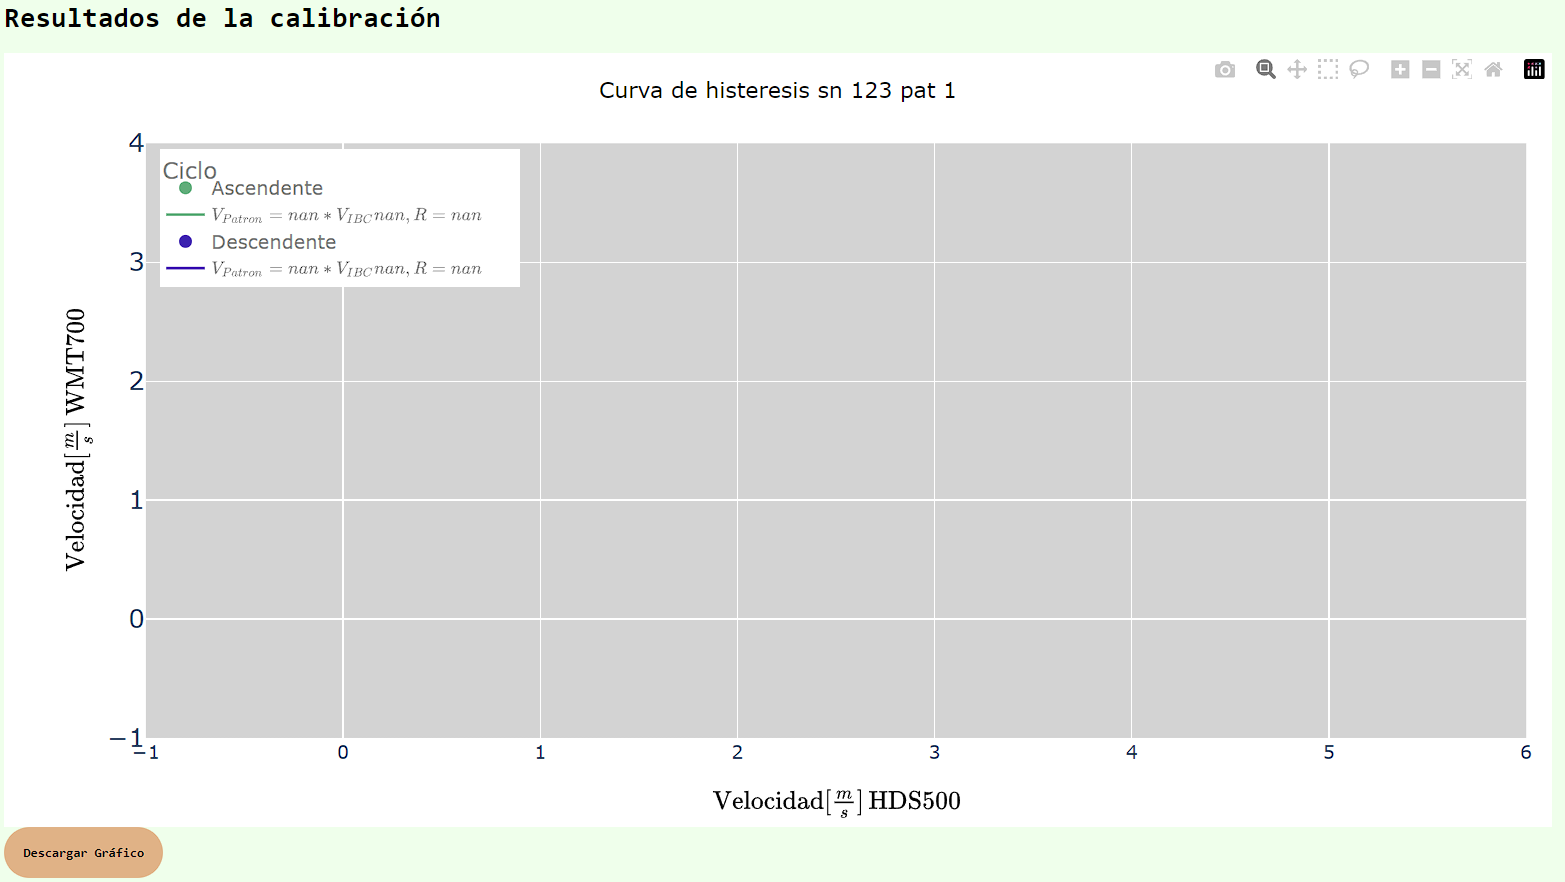
\includegraphics[width=1\linewidth]{Figuras/AplicacionWeb/frontend/curvaHisteris.png}
    \caption{Curva de histéresis.}
    \label{fig:curvaHisteris}
\end{figure}

\begin{figure}[H]
    \centering
    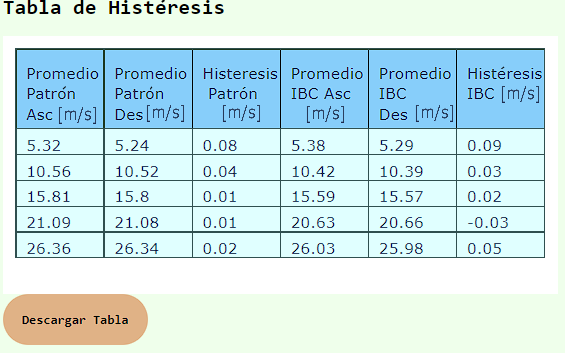
\includegraphics[width=0.55\linewidth]{Figuras/AplicacionWeb/frontend/tablaHisteresis.png}
    \caption{Tabla de valores promedio e histéresis.}
    \label{fig:tablaHisteresis}
\end{figure}

En las Figuras \ref{fig:curvaCalib} y \ref{fig:tablaCalib} se muestran un ejemplo de los espacios donde se cargan los resultados de la calibración. Estos resultados comprenden las curvas de calibración ascendente y descendente con sus respectivas tablas, donde se presentan las correcciones, la incertidumbre combinada y expandida, y los grados de libertad para cada punto.

\begin{figure}[H]
    \centering
    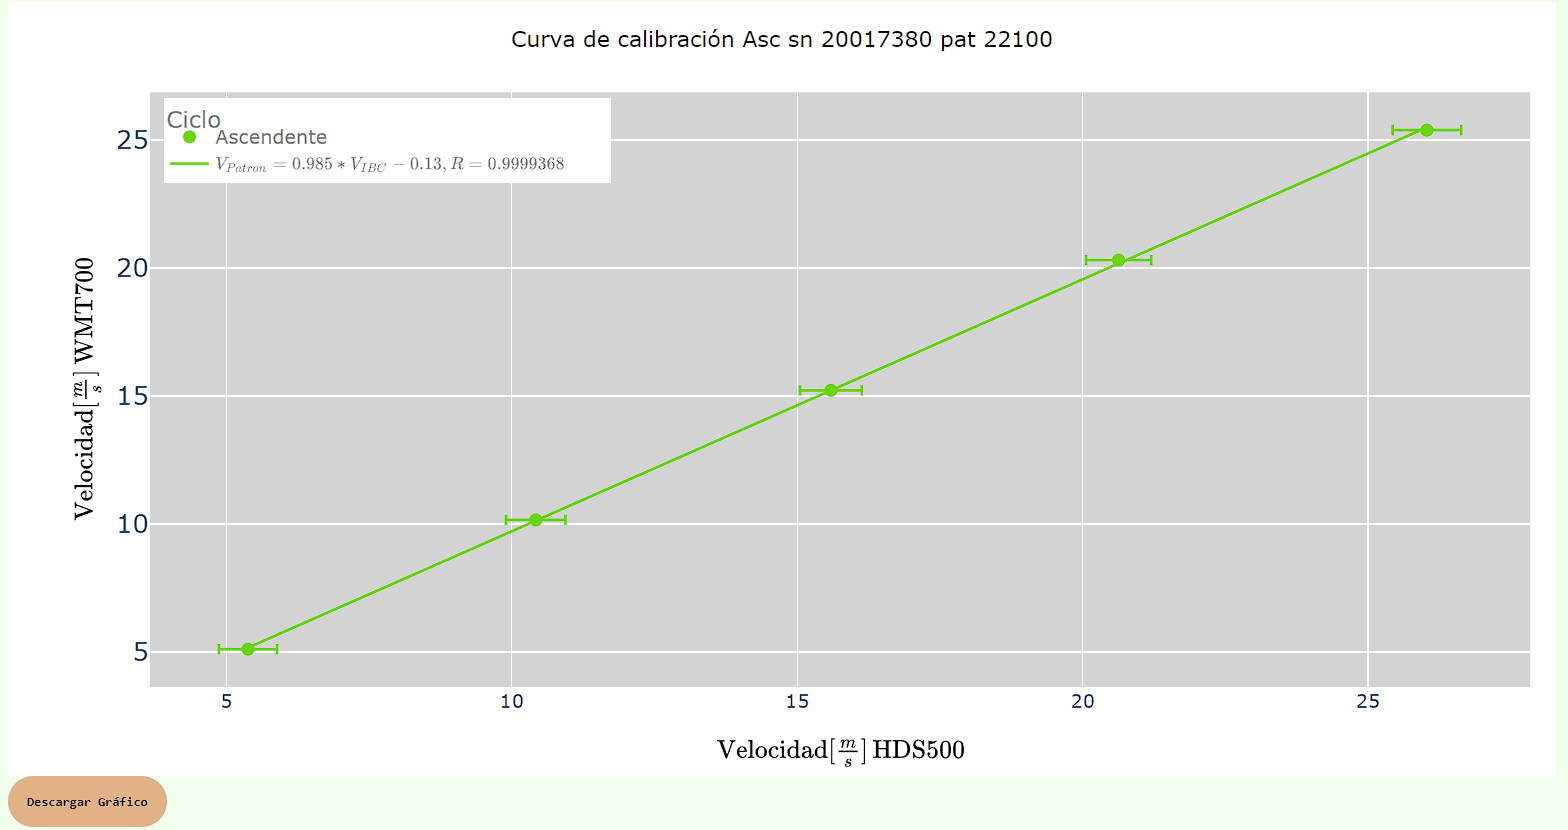
\includegraphics[width=1\linewidth]{Figuras/AplicacionWeb/frontend/curvaCalib.png}
    \caption{Curva de calibración.}
    \label{fig:curvaCalib}
\end{figure}

\begin{figure}[H]
    \centering
    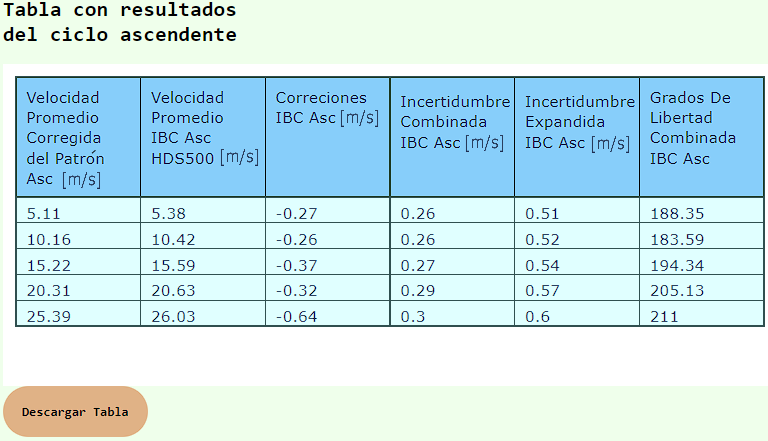
\includegraphics[width=0.7\linewidth]{Figuras/AplicacionWeb/frontend/tablaCalib.png}
    \caption{Tabla de correcciones, incertidumbre y grados de libertad.}
    \label{fig:tablaCalib}
\end{figure}

% mostrar los resultados que muestra el soft como ejemplo usar los del segundo DeltaOHM
%%%%%%%%%%%%%%%%%%%%%%%%%%%%%%%%%%%%%%%%%%%%%%%%%%%%%%%%%%%%%%%%%%%%%%%%%%%%%%%%%%%%%%%%%%%%%%%%%%%%%%%%%%%%%%%%%%%%%%%%
\section{Integración con el hardware}\label{sec:integracionHardware}
(Sacarlo y poner detalles en el banco de medición y configuración del soft del capitulo siguiente)

El software desarrollado interactúa con el hardware, permitiendo al operador configurar de manera sencilla e intuitiva la interfaz eléctrica de los anemómetros, la cadencia de toma de muestras y los puntos de velocidad del viento en el túnel. Se realiza automáticamente el cálculo de incertidumbre y se genera un reporte con los resultados, para el instrumento bajo estudio. Este trabajo estandariza un procedimiento automático para la calibración de sensores de viento ultrasónicos, reduciendo los tiempos operativos, el cálculo manual y los errores sistemáticos, mejorando la calidad en la calibración. Además, el sistema de adquisición, en conjunto con el software y otro sistema de posicionamiento (no incluido en esta tesis), permitirá estudiar en mejor detalle el comportamiento del flujo de aire en la zona de medición.

Los pasos para realizar el proceso de calibración incluyendo el diagrama de la figura \ref{fig:sistemaIntegral} se define a continuación:
\begin{itemize}
    \item Se debe armar el banco de medición, montando los sensores en un soporte dentro del túnel de viento, asegurando que queden fijos y alineados.
    \item Se deben tomar las medidas de posición de los instrumentos respecto a un sistema de referencia.
    \item Se debe calcular el área de bloqueo de cada instrumento, incluyendo su soporte.
    \item Se deben conectar los anemómetros al \textit{datalogger} y alimentar todo el sistema con una fuente de 12 voltios. Además, se debe conectar el {datalogger} a la red LAN local del laboratorio.
    \item Se debe acceder a la interfaz web y configurar los parámetros de calibración.
    \item Se debe iniciar la adquisición de mediciones mediante la interfaz web.
    \item La aplicación Django procesa las solicitudes y envía comandos al \textit{datalogger} a través de \textit{WebSocket}.
    \item El \textit{datalogger} controla el variador de velocidad del motor mediante señales PWM, ajustando el flujo de aire en el túnel de viento.
    \item Los datos de los anemómetros y otros sensores se registran y envían a la aplicación Django.
    \item Terminada las mediciones, el operador debe revisar las mediciones y si son correctas activar el procesamiento.
    \item La aplicación procesa los datos. Primero, calcula el promedio y el desvío estándar de las mediciones para cada punto del escalón. Luego, con esos datos e información ingresada por el usuario, calcula las correcciones e incertidumbres. Finalmente, almacena los resultados en la base de datos.
    \item Los resultados pueden ser visualizados y descargados a través de la interfaz web.
\end{itemize}

\begin{figure}[H]
    \centering
    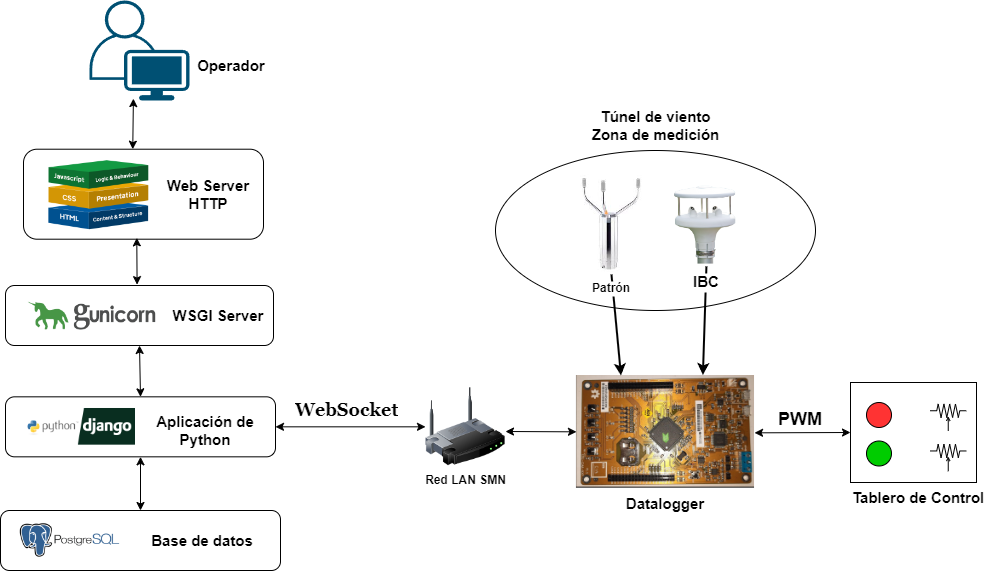
\includegraphics[width=1\linewidth]{Figuras/AplicacionWeb/integracionHardware/DiagramaSistemaDesarrollar.png}
    \caption{Sistema integrado desarrollado en esta tesis.}
    \label{fig:sistemaIntegral}
\end{figure}


% mostrar un diagrama de flujo desde el inicio con el boton calcular incertidumbre hasta la salida de tablas con los reusltados, pasos del proceso de calibración

%-----------------------------------------------------------------------------------------------------
